\documentclass[letterpaper]{book}
\usepackage{makeidx}
\usepackage{graphicx}
\usepackage{multicol}
\usepackage{float}
\usepackage{listings}
\usepackage{color}
\usepackage{ifthen}
\usepackage[table]{xcolor}
\usepackage{textcomp}
\usepackage{alltt}
\usepackage{ifpdf}
\ifpdf
\usepackage[pdftex,
            pagebackref=true,
            colorlinks=true,
            linkcolor=blue,
            unicode
           ]{hyperref}
\else
\usepackage[ps2pdf,
            pagebackref=true,
            colorlinks=true,
            linkcolor=blue,
            unicode
           ]{hyperref}
\usepackage{pspicture}
\fi
\usepackage[utf8]{inputenc}
\usepackage{mathptmx}
\usepackage[scaled=.90]{helvet}
\usepackage{courier}
\usepackage{doxygen}
\lstset{language=C++,inputencoding=utf8,basicstyle=\footnotesize,breaklines=true,breakatwhitespace=true,tabsize=8,numbers=left }
\makeindex
\setcounter{tocdepth}{3}
\renewcommand{\footrulewidth}{0.4pt}
\begin{document}
\hypersetup{pageanchor=false}
\begin{titlepage}
\vspace*{7cm}
\begin{center}
{\Large RJHS FRC Software Documentation \\[1ex]\large 2011 }\\
\vspace*{1cm}
{\large Generated by Doxygen 1.7.3}\\
\vspace*{0.5cm}
{\small Thu Jun 23 2011 17:38:05}\\
\end{center}
\end{titlepage}
\clearemptydoublepage
\pagenumbering{roman}
\tableofcontents
\clearemptydoublepage
\pagenumbering{arabic}
\hypersetup{pageanchor=true}
\chapter{Class Index}
\section{Class List}
Here are the classes, structs, unions and interfaces with brief descriptions:\begin{DoxyCompactList}
\item\contentsline{section}{\hyperlink{class_r_j_f_r_c2011_1_1_autonomous}{Autonomous} (Class managing the \hyperlink{class_r_j_f_r_c2011_1_1_autonomous}{Autonomous} period of the competition )}{\pageref{class_r_j_f_r_c2011_1_1_autonomous}}{}
\item\contentsline{section}{\hyperlink{class_builtin_default_code}{BuiltinDefaultCode} (Our big class that does everything. We didn't bother renaming it )}{\pageref{class_builtin_default_code}}{}
\item\contentsline{section}{\hyperlink{class_r_j_f_r_c2011_1_1_controller}{Controller} (Class abstracting the controller(s) used by our driver(s) )}{\pageref{class_r_j_f_r_c2011_1_1_controller}}{}
\item\contentsline{section}{\hyperlink{class_r_j_f_r_c2011_1_1_drive}{Drive} (Class abstracting the drive system )}{\pageref{class_r_j_f_r_c2011_1_1_drive}}{}
\item\contentsline{section}{\hyperlink{class_r_j_f_r_c2011_1_1_manipulator}{Manipulator} (Abstracts the manipulator )}{\pageref{class_r_j_f_r_c2011_1_1_manipulator}}{}
\item\contentsline{section}{\hyperlink{class_r_j_f_r_c2011_1_1_teleoperated}{Teleoperated} (Class managing robot performance in \hyperlink{class_r_j_f_r_c2011_1_1_teleoperated}{Teleoperated} mode )}{\pageref{class_r_j_f_r_c2011_1_1_teleoperated}}{}
\end{DoxyCompactList}

\chapter{File Index}
\section{File List}
Here is a list of all documented files with brief descriptions:\begin{DoxyCompactList}
\item\contentsline{section}{\hyperlink{_autonomous_8cpp}{Autonomous.cpp} (File containing implementations of functions found in the {\itshape Autonomous\/} class (found in \hyperlink{_autonomous_8h}{Autonomous.h}) )}{\pageref{_autonomous_8cpp}}{}
\item\contentsline{section}{\hyperlink{_autonomous_8h}{Autonomous.h} (File containing definition of {\itshape Autonomous\/} class, which is used within the {\itshape AutomonousPeriodic\/} function in the main program to simplify things )}{\pageref{_autonomous_8h}}{}
\item\contentsline{section}{\hyperlink{_axis_camera_8cpp}{AxisCamera.cpp} (File patching buggy code for the AxisCamera class that causes the robot to freeze )}{\pageref{_axis_camera_8cpp}}{}
\item\contentsline{section}{\hyperlink{_axis_camera_params_8cpp}{AxisCameraParams.cpp} (File patching buggy code for the AxisCameraParams class that causes the robot to freeze. All documentation included was provided by Hurler and/or FIRST, though it was reformatted to be compatible with Doxygen )}{\pageref{_axis_camera_params_8cpp}}{}
\item\contentsline{section}{\hyperlink{_builtin_default_code_8cpp}{BuiltinDefaultCode.cpp} (The file containing the class \hyperlink{class_builtin_default_code}{BuiltinDefaultCode}. We didn't bother changing the name.. )}{\pageref{_builtin_default_code_8cpp}}{}
\item\contentsline{section}{\hyperlink{_controller_8cpp}{Controller.cpp} (File containing implementations of functions found in the {\itshape Controller\/} class (found in \hyperlink{_controller_8h}{Controller.h}) )}{\pageref{_controller_8cpp}}{}
\item\contentsline{section}{\hyperlink{_controller_8h}{Controller.h} (File containing definition of {\itshape Controller\/} class, which is used in both Autonomous and Teleoperated modes to get user input )}{\pageref{_controller_8h}}{}
\item\contentsline{section}{\hyperlink{_drive_8cpp}{Drive.cpp} (File containing definitions of functions declared in class {\itshape Drive\/} (declared in \hyperlink{_drive_8h}{Drive.h}) )}{\pageref{_drive_8cpp}}{}
\item\contentsline{section}{\hyperlink{_drive_8h}{Drive.h} (File containing definition of {\itshape Drive\/} class, which is used in the main program to drive the robot in both Autonomous and Teleoperated modes with no waste of memory )}{\pageref{_drive_8h}}{}
\item\contentsline{section}{\hyperlink{macros_8h}{macros.h} (File containing a bunch of macros to de-\/clutter our other files )}{\pageref{macros_8h}}{}
\item\contentsline{section}{\hyperlink{_manipulator_8cpp}{Manipulator.cpp} (File containing implementations of functions found in the {\itshape Manipulator\/} class (found in \hyperlink{_manipulator_8h}{Manipulator.h}) )}{\pageref{_manipulator_8cpp}}{}
\item\contentsline{section}{\hyperlink{_manipulator_8h}{Manipulator.h} (File containing definition of {\itshape Manipulator\/} class, which is used to simulate the manipulator in both Autonomous and Periodic modes )}{\pageref{_manipulator_8h}}{}
\item\contentsline{section}{\hyperlink{_teleoperated_8cpp}{Teleoperated.cpp} (File containing definitions of functions declared in class {\itshape Teleoperated\/} (declared in \hyperlink{_teleoperated_8h}{Teleoperated.h}) )}{\pageref{_teleoperated_8cpp}}{}
\item\contentsline{section}{\hyperlink{_teleoperated_8h}{Teleoperated.h} (File containing definition of {\itshape Teleoperated\/} class, which is used in the main program during Teleoperated mode to simplify things )}{\pageref{_teleoperated_8h}}{}
\end{DoxyCompactList}

\chapter{Class Documentation}
\hypertarget{class_r_j_f_r_c2011_1_1_autonomous}{
\section{RJFRC2011::Autonomous Class Reference}
\label{class_r_j_f_r_c2011_1_1_autonomous}\index{RJFRC2011::Autonomous@{RJFRC2011::Autonomous}}
}


Class managing the \hyperlink{class_r_j_f_r_c2011_1_1_autonomous}{Autonomous} period of the competition.  




{\ttfamily \#include $<$Autonomous.h$>$}

\subsection*{Public Member Functions}
\begin{DoxyCompactItemize}
\item 
\hyperlink{class_r_j_f_r_c2011_1_1_autonomous_a747bcf35b9790d7b69b14f4303496418}{Autonomous} (\hyperlink{class_r_j_f_r_c2011_1_1_drive}{Drive} $\ast$drive, \hyperlink{class_r_j_f_r_c2011_1_1_manipulator}{Manipulator} $\ast$manip, \hyperlink{class_r_j_f_r_c2011_1_1_controller}{Controller} $\ast$controller, DriverStationLCD $\ast$screen)
\begin{DoxyCompactList}\small\item\em Construct from the addresses of a drive system, a manipulator, a controller, and an LCD screen. \item\end{DoxyCompactList}\item 
\hypertarget{class_r_j_f_r_c2011_1_1_autonomous_a556fc6fc020f18c7bbe6cde03ef81ea4}{
\hyperlink{class_r_j_f_r_c2011_1_1_autonomous_a556fc6fc020f18c7bbe6cde03ef81ea4}{$\sim$Autonomous} ()}
\label{class_r_j_f_r_c2011_1_1_autonomous_a556fc6fc020f18c7bbe6cde03ef81ea4}

\begin{DoxyCompactList}\small\item\em Destructor. Kill stuff. \item\end{DoxyCompactList}\item 
void \hyperlink{class_r_j_f_r_c2011_1_1_autonomous_ab7959f947b71d84b03f53c8e91a542f6}{Go} ()
\begin{DoxyCompactList}\small\item\em State machine function that decides which state to go into. \item\end{DoxyCompactList}\item 
\hypertarget{class_r_j_f_r_c2011_1_1_autonomous_a8cae3af2e3d40459b013583ccec77da6}{
void \hyperlink{class_r_j_f_r_c2011_1_1_autonomous_a8cae3af2e3d40459b013583ccec77da6}{Init} ()}
\label{class_r_j_f_r_c2011_1_1_autonomous_a8cae3af2e3d40459b013583ccec77da6}

\begin{DoxyCompactList}\small\item\em Convenience method. Same as {\itshape \hyperlink{class_r_j_f_r_c2011_1_1_autonomous_a1f04427d07d9569a9f746445c82b8173}{initialState()}\/} \item\end{DoxyCompactList}\item 
\hypertarget{class_r_j_f_r_c2011_1_1_autonomous_ae35c0e29665ed5812645bec8acbbd965}{
void \hyperlink{class_r_j_f_r_c2011_1_1_autonomous_ae35c0e29665ed5812645bec8acbbd965}{printLightSensors} ()}
\label{class_r_j_f_r_c2011_1_1_autonomous_ae35c0e29665ed5812645bec8acbbd965}

\begin{DoxyCompactList}\small\item\em Debug info. Prints the values of lightLeft, lightCenter, and lightRight on the screen. \item\end{DoxyCompactList}\end{DoxyCompactItemize}
\subsection*{Private Member Functions}
\begin{DoxyCompactItemize}
\item 
void \hyperlink{class_r_j_f_r_c2011_1_1_autonomous_a1f04427d07d9569a9f746445c82b8173}{initialState} ()
\begin{DoxyCompactList}\small\item\em The initial state of the robot. \item\end{DoxyCompactList}\item 
void \hyperlink{class_r_j_f_r_c2011_1_1_autonomous_a19885a005434b857e127132a8b871cbe}{checkForLines} ()
\begin{DoxyCompactList}\small\item\em The state in which the robot is looking for tape lines on the floor. \item\end{DoxyCompactList}\item 
void \hyperlink{class_r_j_f_r_c2011_1_1_autonomous_aa3128360e2ac480a3e3ed89e2aeda31b}{move} ()
\begin{DoxyCompactList}\small\item\em State in which the robot moves forward. \item\end{DoxyCompactList}\item 
void \hyperlink{class_r_j_f_r_c2011_1_1_autonomous_acf0141adb70da7e5fe52c5597c0ad34f}{correctRight} ()
\begin{DoxyCompactList}\small\item\em State in which the robot moves slightly to the right. \item\end{DoxyCompactList}\item 
void \hyperlink{class_r_j_f_r_c2011_1_1_autonomous_a04da5791b6204403806e04d6a02ad48f}{correctLeft} ()
\begin{DoxyCompactList}\small\item\em State in which the robot moves slightly to the left. \item\end{DoxyCompactList}\item 
void \hyperlink{class_r_j_f_r_c2011_1_1_autonomous_af0c3a743192b8ba41280999752a1e7da}{placeTube} ()
\begin{DoxyCompactList}\small\item\em State in which the robot ejects the tube (ideally onto a peg) \item\end{DoxyCompactList}\item 
int \hyperlink{class_r_j_f_r_c2011_1_1_autonomous_a71e3ba11ca9e1f84b324a785d1f7985a}{flip} (int x)
\begin{DoxyCompactList}\small\item\em If x is 0, return 1! If x is 1, return 0! \item\end{DoxyCompactList}\end{DoxyCompactItemize}
\subsection*{Private Attributes}
\begin{DoxyCompactItemize}
\item 
\hypertarget{class_r_j_f_r_c2011_1_1_autonomous_a250e8a5a9a38ae5bba7457df67e05462}{
UINT8 \hyperlink{class_r_j_f_r_c2011_1_1_autonomous_a250e8a5a9a38ae5bba7457df67e05462}{lane}}
\label{class_r_j_f_r_c2011_1_1_autonomous_a250e8a5a9a38ae5bba7457df67e05462}

\begin{DoxyCompactList}\small\item\em The starting lane of the robot; 1 for center, 0 for left or right. \item\end{DoxyCompactList}\item 
\hypertarget{class_r_j_f_r_c2011_1_1_autonomous_abcfa4840dd66568b3e263a36d9941bbc}{
char \hyperlink{class_r_j_f_r_c2011_1_1_autonomous_abcfa4840dd66568b3e263a36d9941bbc}{forkDirection}}
\label{class_r_j_f_r_c2011_1_1_autonomous_abcfa4840dd66568b3e263a36d9941bbc}

\begin{DoxyCompactList}\small\item\em If we're in the center lane: do we go left or right at the fork? \item\end{DoxyCompactList}\item 
\hypertarget{class_r_j_f_r_c2011_1_1_autonomous_a15f4f4554332e90259e12aec3baa827b}{
\hyperlink{class_r_j_f_r_c2011_1_1_drive}{Drive} $\ast$ \hyperlink{class_r_j_f_r_c2011_1_1_autonomous_a15f4f4554332e90259e12aec3baa827b}{\_\-drive}}
\label{class_r_j_f_r_c2011_1_1_autonomous_a15f4f4554332e90259e12aec3baa827b}

\begin{DoxyCompactList}\small\item\em Pointer to object abstracting drive mechanism. \item\end{DoxyCompactList}\item 
\hypertarget{class_r_j_f_r_c2011_1_1_autonomous_acaeb4cd9803595987b7fa237247ecd70}{
\hyperlink{class_r_j_f_r_c2011_1_1_manipulator}{Manipulator} $\ast$ \hyperlink{class_r_j_f_r_c2011_1_1_autonomous_acaeb4cd9803595987b7fa237247ecd70}{\_\-manip}}
\label{class_r_j_f_r_c2011_1_1_autonomous_acaeb4cd9803595987b7fa237247ecd70}

\begin{DoxyCompactList}\small\item\em Pointer to object abstracting manipulator. \item\end{DoxyCompactList}\item 
\hypertarget{class_r_j_f_r_c2011_1_1_autonomous_ad5f5bd5da92e33c84b1227d98fe9db47}{
\hyperlink{class_r_j_f_r_c2011_1_1_controller}{Controller} $\ast$ \hyperlink{class_r_j_f_r_c2011_1_1_autonomous_ad5f5bd5da92e33c84b1227d98fe9db47}{\_\-controller}}
\label{class_r_j_f_r_c2011_1_1_autonomous_ad5f5bd5da92e33c84b1227d98fe9db47}

\begin{DoxyCompactList}\small\item\em Pointer to object abstracting controller. \item\end{DoxyCompactList}\item 
\hypertarget{class_r_j_f_r_c2011_1_1_autonomous_a45427a812f865b5d200b2642e53d44b0}{
DriverStationLCD $\ast$ \hyperlink{class_r_j_f_r_c2011_1_1_autonomous_a45427a812f865b5d200b2642e53d44b0}{\_\-screen}}
\label{class_r_j_f_r_c2011_1_1_autonomous_a45427a812f865b5d200b2642e53d44b0}

\begin{DoxyCompactList}\small\item\em Pointer to object representing LCD screen on the Driver Station. Used toprint feedback to the screen. \item\end{DoxyCompactList}\item 
\hypertarget{class_r_j_f_r_c2011_1_1_autonomous_ae6c458fcfb8244e4e112c6a836bb5609}{
DigitalInput $\ast$ \hyperlink{class_r_j_f_r_c2011_1_1_autonomous_ae6c458fcfb8244e4e112c6a836bb5609}{lightSensorLeft}}
\label{class_r_j_f_r_c2011_1_1_autonomous_ae6c458fcfb8244e4e112c6a836bb5609}

\begin{DoxyCompactList}\small\item\em Pointer to object interfacing with leftmost light sensor. \item\end{DoxyCompactList}\item 
\hypertarget{class_r_j_f_r_c2011_1_1_autonomous_a4b9f4445f2514da0e59f9129b1b247d3}{
DigitalInput $\ast$ \hyperlink{class_r_j_f_r_c2011_1_1_autonomous_a4b9f4445f2514da0e59f9129b1b247d3}{lightSensorCenter}}
\label{class_r_j_f_r_c2011_1_1_autonomous_a4b9f4445f2514da0e59f9129b1b247d3}

\begin{DoxyCompactList}\small\item\em Pointer to object interfacing with center light sensor. \item\end{DoxyCompactList}\item 
\hypertarget{class_r_j_f_r_c2011_1_1_autonomous_a8ada7ae26d2b78274febe96a415c7fb0}{
DigitalInput $\ast$ \hyperlink{class_r_j_f_r_c2011_1_1_autonomous_a8ada7ae26d2b78274febe96a415c7fb0}{lightSensorRight}}
\label{class_r_j_f_r_c2011_1_1_autonomous_a8ada7ae26d2b78274febe96a415c7fb0}

\begin{DoxyCompactList}\small\item\em Pointer to object interfacing with rightmost light sensor. \item\end{DoxyCompactList}\item 
\hypertarget{class_r_j_f_r_c2011_1_1_autonomous_afa181f57e25cab35aa5eeffdbc1bd43d}{
DigitalInput $\ast$ \hyperlink{class_r_j_f_r_c2011_1_1_autonomous_afa181f57e25cab35aa5eeffdbc1bd43d}{autonomousLaneSwitch}}
\label{class_r_j_f_r_c2011_1_1_autonomous_afa181f57e25cab35aa5eeffdbc1bd43d}

\begin{DoxyCompactList}\small\item\em Physical switch controlling which lane our robot starts out in. \item\end{DoxyCompactList}\item 
\hypertarget{class_r_j_f_r_c2011_1_1_autonomous_aff3688fd6c4119516863947014e17aca}{
DigitalInput $\ast$ \hyperlink{class_r_j_f_r_c2011_1_1_autonomous_aff3688fd6c4119516863947014e17aca}{autonomousForkSwitch}}
\label{class_r_j_f_r_c2011_1_1_autonomous_aff3688fd6c4119516863947014e17aca}

\begin{DoxyCompactList}\small\item\em Physical switch controlling which direction our robot is to take if it's in the center lane. \item\end{DoxyCompactList}\end{DoxyCompactItemize}


\subsection{Detailed Description}
Class managing the \hyperlink{class_r_j_f_r_c2011_1_1_autonomous}{Autonomous} period of the competition. Manages a \char`\"{}state machine\char`\"{} (essentially a {\itshape switch\/} block) that defines which of a number of \char`\"{}states\char`\"{} to execute based on inputs from three light sensors. These states are: check light sensors, move, correct left, correct right, place tube. 

\subsection{Constructor \& Destructor Documentation}
\hypertarget{class_r_j_f_r_c2011_1_1_autonomous_a747bcf35b9790d7b69b14f4303496418}{
\index{RJFRC2011::Autonomous@{RJFRC2011::Autonomous}!Autonomous@{Autonomous}}
\index{Autonomous@{Autonomous}!RJFRC2011::Autonomous@{RJFRC2011::Autonomous}}
\subsubsection[{Autonomous}]{\setlength{\rightskip}{0pt plus 5cm}RJFRC2011::Autonomous::Autonomous (
\begin{DoxyParamCaption}
\item[{{\bf Drive} $\ast$}]{drive, }
\item[{{\bf Manipulator} $\ast$}]{manip, }
\item[{{\bf Controller} $\ast$}]{controller, }
\item[{DriverStationLCD $\ast$}]{screen}
\end{DoxyParamCaption}
)}}
\label{class_r_j_f_r_c2011_1_1_autonomous_a747bcf35b9790d7b69b14f4303496418}


Construct from the addresses of a drive system, a manipulator, a controller, and an LCD screen. 


\begin{DoxyParams}{Parameters}
{\em drive} & Pointer to a {\itshape \hyperlink{class_r_j_f_r_c2011_1_1_drive}{Drive}\/} variable that will be used in both \hyperlink{class_r_j_f_r_c2011_1_1_autonomous}{Autonomous} and \hyperlink{class_r_j_f_r_c2011_1_1_teleoperated}{Teleoperated} periods. \\
\hline
{\em manip} & Pointer to a {\itshape \hyperlink{class_r_j_f_r_c2011_1_1_manipulator}{Manipulator}\/} variable that will be used in both \hyperlink{class_r_j_f_r_c2011_1_1_autonomous}{Autonomous} and \hyperlink{class_r_j_f_r_c2011_1_1_teleoperated}{Teleoperated} periods. \\
\hline
{\em controller} & Pointer to a {\itshape \hyperlink{class_r_j_f_r_c2011_1_1_controller}{Controller}\/} variable that will be used in both \hyperlink{class_r_j_f_r_c2011_1_1_autonomous}{Autonomous} and \hyperlink{class_r_j_f_r_c2011_1_1_teleoperated}{Teleoperated} periods. \\
\hline
{\em screen} & Pointer to a {\itshape DriverStationLCD\/} variable that will be used in \hyperlink{class_r_j_f_r_c2011_1_1_autonomous}{Autonomous}, \hyperlink{class_r_j_f_r_c2011_1_1_teleoperated}{Teleoperated}, and Disabled periods to write to the screen. \\
\hline
\end{DoxyParams}


\subsection{Member Function Documentation}
\hypertarget{class_r_j_f_r_c2011_1_1_autonomous_a19885a005434b857e127132a8b871cbe}{
\index{RJFRC2011::Autonomous@{RJFRC2011::Autonomous}!checkForLines@{checkForLines}}
\index{checkForLines@{checkForLines}!RJFRC2011::Autonomous@{RJFRC2011::Autonomous}}
\subsubsection[{checkForLines}]{\setlength{\rightskip}{0pt plus 5cm}void RJFRC2011::Autonomous::checkForLines (
\begin{DoxyParamCaption}
{}
\end{DoxyParamCaption}
)\hspace{0.3cm}{\ttfamily  \mbox{[}private\mbox{]}}}}
\label{class_r_j_f_r_c2011_1_1_autonomous_a19885a005434b857e127132a8b871cbe}


The state in which the robot is looking for tape lines on the floor. 

Read input from the 3 light sensors and store the results in three variables. \hypertarget{class_r_j_f_r_c2011_1_1_autonomous_a04da5791b6204403806e04d6a02ad48f}{
\index{RJFRC2011::Autonomous@{RJFRC2011::Autonomous}!correctLeft@{correctLeft}}
\index{correctLeft@{correctLeft}!RJFRC2011::Autonomous@{RJFRC2011::Autonomous}}
\subsubsection[{correctLeft}]{\setlength{\rightskip}{0pt plus 5cm}void RJFRC2011::Autonomous::correctLeft (
\begin{DoxyParamCaption}
{}
\end{DoxyParamCaption}
)\hspace{0.3cm}{\ttfamily  \mbox{[}private\mbox{]}}}}
\label{class_r_j_f_r_c2011_1_1_autonomous_a04da5791b6204403806e04d6a02ad48f}


State in which the robot moves slightly to the left. 

Print to the screen that we're in {\itshape \hyperlink{class_r_j_f_r_c2011_1_1_autonomous_a04da5791b6204403806e04d6a02ad48f}{correctLeft()}\/} and turn left by driving the left wheels at -\/.15 and the right wheels at {\itshape AUTO\_\-TURN\_\-SPEED\/}. \hypertarget{class_r_j_f_r_c2011_1_1_autonomous_acf0141adb70da7e5fe52c5597c0ad34f}{
\index{RJFRC2011::Autonomous@{RJFRC2011::Autonomous}!correctRight@{correctRight}}
\index{correctRight@{correctRight}!RJFRC2011::Autonomous@{RJFRC2011::Autonomous}}
\subsubsection[{correctRight}]{\setlength{\rightskip}{0pt plus 5cm}void RJFRC2011::Autonomous::correctRight (
\begin{DoxyParamCaption}
{}
\end{DoxyParamCaption}
)\hspace{0.3cm}{\ttfamily  \mbox{[}private\mbox{]}}}}
\label{class_r_j_f_r_c2011_1_1_autonomous_acf0141adb70da7e5fe52c5597c0ad34f}


State in which the robot moves slightly to the right. 

Print to the screen that we're in {\itshape \hyperlink{class_r_j_f_r_c2011_1_1_autonomous_acf0141adb70da7e5fe52c5597c0ad34f}{correctRight()}\/} and turn right by driving the left wheels at {\itshape AUTO\_\-TURN\_\-SPEED\/} and the right wheels at -\/.15. \hypertarget{class_r_j_f_r_c2011_1_1_autonomous_a71e3ba11ca9e1f84b324a785d1f7985a}{
\index{RJFRC2011::Autonomous@{RJFRC2011::Autonomous}!flip@{flip}}
\index{flip@{flip}!RJFRC2011::Autonomous@{RJFRC2011::Autonomous}}
\subsubsection[{flip}]{\setlength{\rightskip}{0pt plus 5cm}int RJFRC2011::Autonomous::flip (
\begin{DoxyParamCaption}
\item[{int}]{x}
\end{DoxyParamCaption}
)\hspace{0.3cm}{\ttfamily  \mbox{[}private\mbox{]}}}}
\label{class_r_j_f_r_c2011_1_1_autonomous_a71e3ba11ca9e1f84b324a785d1f7985a}


If x is 0, return 1! If x is 1, return 0! 


\begin{DoxyParams}{Parameters}
{\em x} & The value to be flipped \\
\hline
\end{DoxyParams}
\begin{DoxyReturn}{Returns}
The flipped value 
\end{DoxyReturn}
\hypertarget{class_r_j_f_r_c2011_1_1_autonomous_ab7959f947b71d84b03f53c8e91a542f6}{
\index{RJFRC2011::Autonomous@{RJFRC2011::Autonomous}!Go@{Go}}
\index{Go@{Go}!RJFRC2011::Autonomous@{RJFRC2011::Autonomous}}
\subsubsection[{Go}]{\setlength{\rightskip}{0pt plus 5cm}void RJFRC2011::Autonomous::Go (
\begin{DoxyParamCaption}
{}
\end{DoxyParamCaption}
)}}
\label{class_r_j_f_r_c2011_1_1_autonomous_ab7959f947b71d84b03f53c8e91a542f6}


State machine function that decides which state to go into. 

Operates on the {\itshape lightX\/} variables to tell where the line is, with 0 indicating that the sensor saw nothing and 1 indicating that the sensor detected something (ideally the tape). We then use a sereis of {\itshape if\/} statements to change to the appropriate state. \hypertarget{class_r_j_f_r_c2011_1_1_autonomous_a1f04427d07d9569a9f746445c82b8173}{
\index{RJFRC2011::Autonomous@{RJFRC2011::Autonomous}!initialState@{initialState}}
\index{initialState@{initialState}!RJFRC2011::Autonomous@{RJFRC2011::Autonomous}}
\subsubsection[{initialState}]{\setlength{\rightskip}{0pt plus 5cm}void RJFRC2011::Autonomous::initialState (
\begin{DoxyParamCaption}
{}
\end{DoxyParamCaption}
)\hspace{0.3cm}{\ttfamily  \mbox{[}private\mbox{]}}}}
\label{class_r_j_f_r_c2011_1_1_autonomous_a1f04427d07d9569a9f746445c82b8173}


The initial state of the robot. 

Read input from the switches and set variables accordingly. If lane switch is off, we're in a side lane; if it's on, we're in the center one. If we're in the center, read the second fork switch: if it's on, go left; if not, go right. \hypertarget{class_r_j_f_r_c2011_1_1_autonomous_aa3128360e2ac480a3e3ed89e2aeda31b}{
\index{RJFRC2011::Autonomous@{RJFRC2011::Autonomous}!move@{move}}
\index{move@{move}!RJFRC2011::Autonomous@{RJFRC2011::Autonomous}}
\subsubsection[{move}]{\setlength{\rightskip}{0pt plus 5cm}void RJFRC2011::Autonomous::move (
\begin{DoxyParamCaption}
{}
\end{DoxyParamCaption}
)\hspace{0.3cm}{\ttfamily  \mbox{[}private\mbox{]}}}}
\label{class_r_j_f_r_c2011_1_1_autonomous_aa3128360e2ac480a3e3ed89e2aeda31b}


State in which the robot moves forward. 

Print to the screen that we're in {\itshape \hyperlink{class_r_j_f_r_c2011_1_1_autonomous_aa3128360e2ac480a3e3ed89e2aeda31b}{move()}\/} and drive forward at {\itshape AUTO\_\-DRIVE\_\-SPEED\/} \hypertarget{class_r_j_f_r_c2011_1_1_autonomous_af0c3a743192b8ba41280999752a1e7da}{
\index{RJFRC2011::Autonomous@{RJFRC2011::Autonomous}!placeTube@{placeTube}}
\index{placeTube@{placeTube}!RJFRC2011::Autonomous@{RJFRC2011::Autonomous}}
\subsubsection[{placeTube}]{\setlength{\rightskip}{0pt plus 5cm}void RJFRC2011::Autonomous::placeTube (
\begin{DoxyParamCaption}
{}
\end{DoxyParamCaption}
)\hspace{0.3cm}{\ttfamily  \mbox{[}private\mbox{]}}}}
\label{class_r_j_f_r_c2011_1_1_autonomous_af0c3a743192b8ba41280999752a1e7da}


State in which the robot ejects the tube (ideally onto a peg) 

Brake the robot to a stop, print that we're in {\itshape \hyperlink{class_r_j_f_r_c2011_1_1_autonomous_af0c3a743192b8ba41280999752a1e7da}{placeTube()}\/}, and run the ejection wheels for one second. 

The documentation for this class was generated from the following files:\begin{DoxyCompactItemize}
\item 
\hyperlink{_autonomous_8h}{Autonomous.h}\item 
\hyperlink{_autonomous_8cpp}{Autonomous.cpp}\end{DoxyCompactItemize}

\hypertarget{class_builtin_default_code}{
\section{BuiltinDefaultCode Class Reference}
\label{class_builtin_default_code}\index{BuiltinDefaultCode@{BuiltinDefaultCode}}
}


Our big class that does everything. We didn't bother renaming it.  




Collaboration diagram for BuiltinDefaultCode:
\nopagebreak
\begin{figure}[H]
\begin{center}
\leavevmode
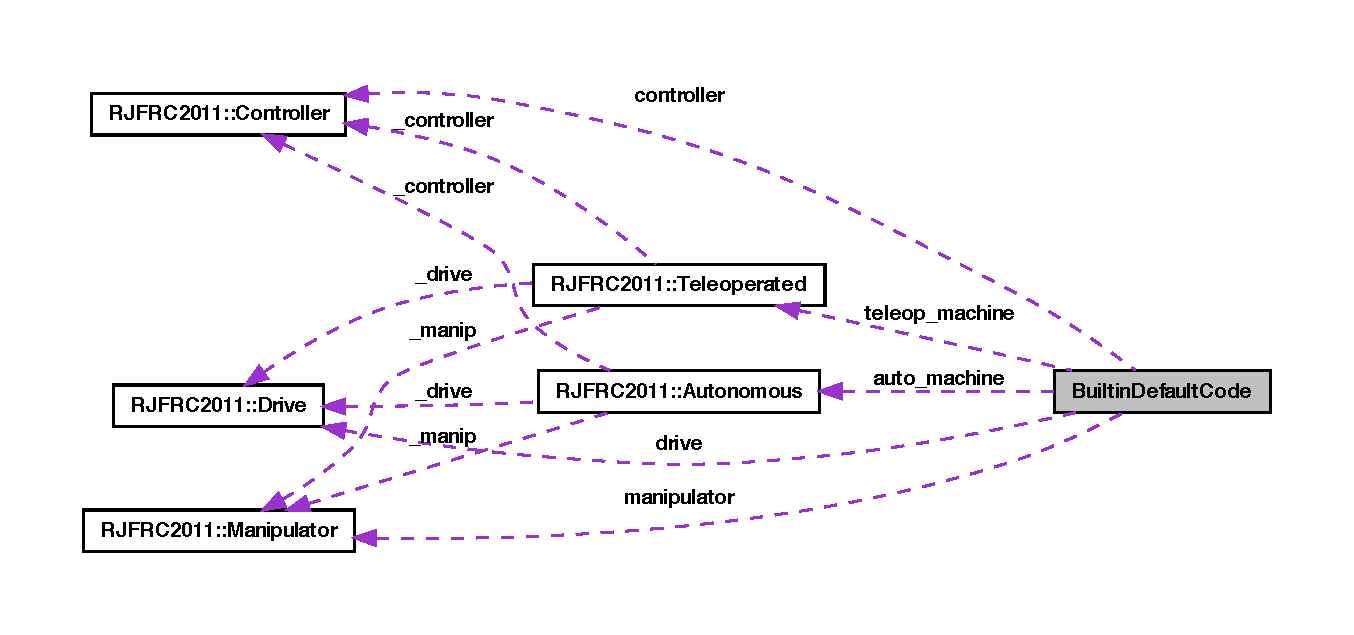
\includegraphics[width=400pt]{class_builtin_default_code__coll__graph}
\end{center}
\end{figure}
\subsection*{Public Member Functions}
\begin{DoxyCompactItemize}
\item 
\hyperlink{class_builtin_default_code_a5f72b929d98fe4193e1a7d8e351a7837}{BuiltinDefaultCode} (void)
\begin{DoxyCompactList}\small\item\em Constructor. \item\end{DoxyCompactList}\item 
\hypertarget{class_builtin_default_code_a04c696dab5af274ca086d8903eb02134}{
\hyperlink{class_builtin_default_code_a04c696dab5af274ca086d8903eb02134}{$\sim$BuiltinDefaultCode} ()}
\label{class_builtin_default_code_a04c696dab5af274ca086d8903eb02134}

\begin{DoxyCompactList}\small\item\em Destructor. Called when a class object expires. Used so we don't waste memory. \item\end{DoxyCompactList}\item 
\hypertarget{class_builtin_default_code_a522b7e1b11f160868900a01a7f5609b6}{
void \hyperlink{class_builtin_default_code_a522b7e1b11f160868900a01a7f5609b6}{RobotInit} (void)}
\label{class_builtin_default_code_a522b7e1b11f160868900a01a7f5609b6}

\begin{DoxyCompactList}\small\item\em Actions which would be performed once (and only once) upon initialization of the robot. \item\end{DoxyCompactList}\item 
\hypertarget{class_builtin_default_code_a1df5e366a588086aedab2510393a9ac6}{
void \hyperlink{class_builtin_default_code_a1df5e366a588086aedab2510393a9ac6}{DisabledInit} (void)}
\label{class_builtin_default_code_a1df5e366a588086aedab2510393a9ac6}

\begin{DoxyCompactList}\small\item\em Code called at the beginning of Disabled Mode. \item\end{DoxyCompactList}\item 
\hypertarget{class_builtin_default_code_a727ebabf0678af822d53f90f96bfd679}{
void \hyperlink{class_builtin_default_code_a727ebabf0678af822d53f90f96bfd679}{AutonomousInit} (void)}
\label{class_builtin_default_code_a727ebabf0678af822d53f90f96bfd679}

\begin{DoxyCompactList}\small\item\em Code called at the beginning of Autonomous Mode. \item\end{DoxyCompactList}\item 
\hypertarget{class_builtin_default_code_ab3d70e0754e54bab03b130e6c042e0b5}{
void \hyperlink{class_builtin_default_code_ab3d70e0754e54bab03b130e6c042e0b5}{TeleopInit} (void)}
\label{class_builtin_default_code_ab3d70e0754e54bab03b130e6c042e0b5}

\begin{DoxyCompactList}\small\item\em Code called at the beginning of Teleoperated Mode. \item\end{DoxyCompactList}\item 
\hypertarget{class_builtin_default_code_a504e7d9b01a66635c31597f9a58cf478}{
void \hyperlink{class_builtin_default_code_a504e7d9b01a66635c31597f9a58cf478}{DisabledPeriodic} (void)}
\label{class_builtin_default_code_a504e7d9b01a66635c31597f9a58cf478}

\begin{DoxyCompactList}\small\item\em The code called in a loop during Disabled Mode. Left as the default, minus the loop counter. \item\end{DoxyCompactList}\item 
\hypertarget{class_builtin_default_code_a26da787e2abf683077e266ad44049ca0}{
void \hyperlink{class_builtin_default_code_a26da787e2abf683077e266ad44049ca0}{AutonomousPeriodic} (void)}
\label{class_builtin_default_code_a26da787e2abf683077e266ad44049ca0}

\begin{DoxyCompactList}\small\item\em The code called in a loop during Autonomous Mode. \item\end{DoxyCompactList}\item 
\hypertarget{class_builtin_default_code_a79dd68c3dba134d041413df30862aae2}{
void \hyperlink{class_builtin_default_code_a79dd68c3dba134d041413df30862aae2}{TeleopPeriodic} (void)}
\label{class_builtin_default_code_a79dd68c3dba134d041413df30862aae2}

\begin{DoxyCompactList}\small\item\em The code called in a loop during Teleoperated Mode. \item\end{DoxyCompactList}\end{DoxyCompactItemize}
\subsection*{Private Attributes}
\begin{DoxyCompactItemize}
\item 
\hypertarget{class_builtin_default_code_a2d4ed2369361dcd5b02e74dac9b3f4dd}{
\hyperlink{class_r_j_f_r_c2011_1_1_drive}{Drive} $\ast$ \hyperlink{class_builtin_default_code_a2d4ed2369361dcd5b02e74dac9b3f4dd}{drive}}
\label{class_builtin_default_code_a2d4ed2369361dcd5b02e74dac9b3f4dd}

\begin{DoxyCompactList}\small\item\em Class abstracting drive system. \item\end{DoxyCompactList}\item 
\hypertarget{class_builtin_default_code_ac2ed56fdb661e5c24cd9b012f9d09b63}{
\hyperlink{class_r_j_f_r_c2011_1_1_manipulator}{Manipulator} $\ast$ \hyperlink{class_builtin_default_code_ac2ed56fdb661e5c24cd9b012f9d09b63}{manipulator}}
\label{class_builtin_default_code_ac2ed56fdb661e5c24cd9b012f9d09b63}

\begin{DoxyCompactList}\small\item\em Class abstracting manipulator. \item\end{DoxyCompactList}\item 
\hypertarget{class_builtin_default_code_af8e1d3aaa175d9d8091438a00b4b1556}{
\hyperlink{class_r_j_f_r_c2011_1_1_controller}{Controller} $\ast$ \hyperlink{class_builtin_default_code_af8e1d3aaa175d9d8091438a00b4b1556}{controller}}
\label{class_builtin_default_code_af8e1d3aaa175d9d8091438a00b4b1556}

\begin{DoxyCompactList}\small\item\em Class abstracting the controller. \item\end{DoxyCompactList}\item 
\hypertarget{class_builtin_default_code_ac09bfa871751a5c092c1db9cb3ad37e9}{
DriverStationLCD $\ast$ \hyperlink{class_builtin_default_code_ac09bfa871751a5c092c1db9cb3ad37e9}{screen}}
\label{class_builtin_default_code_ac09bfa871751a5c092c1db9cb3ad37e9}

\begin{DoxyCompactList}\small\item\em The screen. Yup. \item\end{DoxyCompactList}\item 
\hypertarget{class_builtin_default_code_a39f6383c7d191eeca78ab4a9865d6664}{
DriverStation $\ast$ \hyperlink{class_builtin_default_code_a39f6383c7d191eeca78ab4a9865d6664}{ds}}
\label{class_builtin_default_code_a39f6383c7d191eeca78ab4a9865d6664}

\begin{DoxyCompactList}\small\item\em Driver Station object; used so we can send info back to the user (at least, in theory) \item\end{DoxyCompactList}\item 
\hypertarget{class_builtin_default_code_aef2c4c3029fc5446af5117125ffdc555}{
AxisCamera $\ast$ \hyperlink{class_builtin_default_code_aef2c4c3029fc5446af5117125ffdc555}{cam}}
\label{class_builtin_default_code_aef2c4c3029fc5446af5117125ffdc555}

\begin{DoxyCompactList}\small\item\em Our rear-\/mounted camera, used to see stuff in style. \item\end{DoxyCompactList}\item 
\hypertarget{class_builtin_default_code_a23fafbc7100e3b5b50408d010b5f609b}{
\hyperlink{class_r_j_f_r_c2011_1_1_autonomous}{Autonomous} $\ast$ \hyperlink{class_builtin_default_code_a23fafbc7100e3b5b50408d010b5f609b}{auto\_\-machine}}
\label{class_builtin_default_code_a23fafbc7100e3b5b50408d010b5f609b}

\begin{DoxyCompactList}\small\item\em Class running the Autonomous period. \item\end{DoxyCompactList}\item 
\hypertarget{class_builtin_default_code_ad31f83ef30fd7bbb3bbe22895dfb9c99}{
\hyperlink{class_r_j_f_r_c2011_1_1_teleoperated}{Teleoperated} $\ast$ \hyperlink{class_builtin_default_code_ad31f83ef30fd7bbb3bbe22895dfb9c99}{teleop\_\-machine}}
\label{class_builtin_default_code_ad31f83ef30fd7bbb3bbe22895dfb9c99}

\begin{DoxyCompactList}\small\item\em Class running the Teleoperated period. \item\end{DoxyCompactList}\item 
\hypertarget{class_builtin_default_code_aaf59606d706817c312686afcd1f8f527}{
Timer $\ast$ \hyperlink{class_builtin_default_code_aaf59606d706817c312686afcd1f8f527}{timer}}
\label{class_builtin_default_code_aaf59606d706817c312686afcd1f8f527}

\begin{DoxyCompactList}\small\item\em Used to time movements in Autonomous. \item\end{DoxyCompactList}\end{DoxyCompactItemize}


\subsection{Detailed Description}
Our big class that does everything. We didn't bother renaming it. \hyperlink{class_builtin_default_code}{BuiltinDefaultCode} is technically the name of the example class that we first opened, but once we started coding we realized that we couldn't rename the project and didn't want to reconfigure all the build settings from scratch. So here we are. 

\subsection{Constructor \& Destructor Documentation}
\hypertarget{class_builtin_default_code_a5f72b929d98fe4193e1a7d8e351a7837}{
\index{BuiltinDefaultCode@{BuiltinDefaultCode}!BuiltinDefaultCode@{BuiltinDefaultCode}}
\index{BuiltinDefaultCode@{BuiltinDefaultCode}!BuiltinDefaultCode@{BuiltinDefaultCode}}
\subsubsection[{BuiltinDefaultCode}]{\setlength{\rightskip}{0pt plus 5cm}BuiltinDefaultCode::BuiltinDefaultCode (
\begin{DoxyParamCaption}
\item[{void}]{}
\end{DoxyParamCaption}
)\hspace{0.3cm}{\ttfamily  \mbox{[}inline\mbox{]}}}}
\label{class_builtin_default_code_a5f72b929d98fe4193e1a7d8e351a7837}


Constructor. 

Set up things before robot does anything; mostly this allocates memory for things. 

The documentation for this class was generated from the following file:\begin{DoxyCompactItemize}
\item 
\hyperlink{_builtin_default_code_8cpp}{BuiltinDefaultCode.cpp}\end{DoxyCompactItemize}

\hypertarget{class_r_j_f_r_c2011_1_1_controller}{
\section{RJFRC2011::Controller Class Reference}
\label{class_r_j_f_r_c2011_1_1_controller}\index{RJFRC2011::Controller@{RJFRC2011::Controller}}
}


Class abstracting the controller(s) used by our driver(s)  




{\ttfamily \#include $<$Controller.h$>$}

\subsection*{Public Member Functions}
\begin{DoxyCompactItemize}
\item 
\hyperlink{class_r_j_f_r_c2011_1_1_controller_ace98163d9d5fc6deec6bdc294c2ef593}{Controller} ()
\begin{DoxyCompactList}\small\item\em Constructor. \item\end{DoxyCompactList}\item 
\hypertarget{class_r_j_f_r_c2011_1_1_controller_a56d34929cf6b8e9f277728404ff67d5f}{
\hyperlink{class_r_j_f_r_c2011_1_1_controller_a56d34929cf6b8e9f277728404ff67d5f}{$\sim$Controller} ()}
\label{class_r_j_f_r_c2011_1_1_controller_a56d34929cf6b8e9f277728404ff67d5f}

\begin{DoxyCompactList}\small\item\em Destructor. Kill stuff. \item\end{DoxyCompactList}\item 
float \hyperlink{class_r_j_f_r_c2011_1_1_controller_afc9c35671f9791605d7c6a55d5c0375b}{getManipulatorElevation} ()
\begin{DoxyCompactList}\small\item\em Get user-\/requested manipulator elevation. \item\end{DoxyCompactList}\item 
float \hyperlink{class_r_j_f_r_c2011_1_1_controller_abee0ec4f9aa51ded688943dab941221e}{getDriveSpeed} ()
\begin{DoxyCompactList}\small\item\em Get user-\/requested drive speed. \item\end{DoxyCompactList}\item 
float \hyperlink{class_r_j_f_r_c2011_1_1_controller_a08f649d3f9e8cd04e4096186949b7920}{getDriveTurn} ()
\begin{DoxyCompactList}\small\item\em Get user-\/requested drive turn speed. \item\end{DoxyCompactList}\item 
int \hyperlink{class_r_j_f_r_c2011_1_1_controller_aac5a08c91980af6d162c0661b5bfde8d}{getMinibotSwitches} ()
\begin{DoxyCompactList}\small\item\em Get user-\/requested minibot shelf action (in/out). \item\end{DoxyCompactList}\end{DoxyCompactItemize}
\subsection*{Static Public Member Functions}
\begin{DoxyCompactItemize}
\item 
static int \hyperlink{class_r_j_f_r_c2011_1_1_controller_a19a25438de68dc0284862e2347bb576c}{getManipulatorAction} ()
\begin{DoxyCompactList}\small\item\em Get user-\/requested manipulator action (input, rotate, or eject). \item\end{DoxyCompactList}\end{DoxyCompactItemize}
\subsection*{Private Member Functions}
\begin{DoxyCompactItemize}
\item 
float \hyperlink{class_r_j_f_r_c2011_1_1_controller_ac2c90813eff8dbebc38210c605d4b2d2}{abs} (float initial)
\begin{DoxyCompactList}\small\item\em Absolute value of a float, since I'm not sure if we can import the $<$cmath$>$ library onto the cRIO. EDIT: turns out we can, but I'll leave this here to conserve memory. \item\end{DoxyCompactList}\item 
float \hyperlink{class_r_j_f_r_c2011_1_1_controller_a70def9152e72c1745dccce7c3121f5ac}{expo} (float x, float a)
\begin{DoxyCompactList}\small\item\em An exponential function used to make joysticks less sensitive near the center and more sensitive towards the edges. \item\end{DoxyCompactList}\item 
float \hyperlink{class_r_j_f_r_c2011_1_1_controller_ac2e4beb60add909ce7c0716551501fcf}{normalize} (float joyVal, float min, float max)
\begin{DoxyCompactList}\small\item\em A function that \char`\"{}normalizes\char`\"{} inputs from the joysticks (because they don't give perfect -\/1.0 to 1.0 values). \item\end{DoxyCompactList}\end{DoxyCompactItemize}
\subsection*{Private Attributes}
\begin{DoxyCompactItemize}
\item 
\hypertarget{class_r_j_f_r_c2011_1_1_controller_af6484856a3ffd56d9201186d3f96341a}{
Joystick $\ast$ \hyperlink{class_r_j_f_r_c2011_1_1_controller_af6484856a3ffd56d9201186d3f96341a}{\_\-controller}}
\label{class_r_j_f_r_c2011_1_1_controller_af6484856a3ffd56d9201186d3f96341a}

\begin{DoxyCompactList}\small\item\em Object abstracting our InterLink Elite controller, which WIPLib seems to think is a joystick. \item\end{DoxyCompactList}\item 
\hypertarget{class_r_j_f_r_c2011_1_1_controller_aa9347538d57c8e3ee63610bdfe4fea9e}{
Joystick $\ast$ \hyperlink{class_r_j_f_r_c2011_1_1_controller_aa9347538d57c8e3ee63610bdfe4fea9e}{\_\-joystick}}
\label{class_r_j_f_r_c2011_1_1_controller_aa9347538d57c8e3ee63610bdfe4fea9e}

\begin{DoxyCompactList}\small\item\em Object abstracting our legitimate Logitech Attack3 joystick. \item\end{DoxyCompactList}\end{DoxyCompactItemize}


\subsection{Detailed Description}
Class abstracting the controller(s) used by our driver(s) Get input from a pair of joysticks (one of which is physically a flight simulator controller) and return those inputs. A class like this is useful because we can modify a few lines of code to change the inputs for functions throughout the entire code. 

\subsection{Constructor \& Destructor Documentation}
\hypertarget{class_r_j_f_r_c2011_1_1_controller_ace98163d9d5fc6deec6bdc294c2ef593}{
\index{RJFRC2011::Controller@{RJFRC2011::Controller}!Controller@{Controller}}
\index{Controller@{Controller}!RJFRC2011::Controller@{RJFRC2011::Controller}}
\subsubsection[{Controller}]{\setlength{\rightskip}{0pt plus 5cm}RJFRC2011::Controller::Controller (
\begin{DoxyParamCaption}
{}
\end{DoxyParamCaption}
)}}
\label{class_r_j_f_r_c2011_1_1_controller_ace98163d9d5fc6deec6bdc294c2ef593}


Constructor. 

Basically, initialize the controllers to USB ports 1 and 2. 

\subsection{Member Function Documentation}
\hypertarget{class_r_j_f_r_c2011_1_1_controller_ac2c90813eff8dbebc38210c605d4b2d2}{
\index{RJFRC2011::Controller@{RJFRC2011::Controller}!abs@{abs}}
\index{abs@{abs}!RJFRC2011::Controller@{RJFRC2011::Controller}}
\subsubsection[{abs}]{\setlength{\rightskip}{0pt plus 5cm}float RJFRC2011::Controller::abs (
\begin{DoxyParamCaption}
\item[{float}]{initial}
\end{DoxyParamCaption}
)\hspace{0.3cm}{\ttfamily  \mbox{[}private\mbox{]}}}}
\label{class_r_j_f_r_c2011_1_1_controller_ac2c90813eff8dbebc38210c605d4b2d2}


Absolute value of a float, since I'm not sure if we can import the $<$cmath$>$ library onto the cRIO. EDIT: turns out we can, but I'll leave this here to conserve memory. 


\begin{DoxyParams}{Parameters}
{\em initial} & the initial value \\
\hline
\end{DoxyParams}
\begin{DoxyReturn}{Returns}
the absolute value of the passed value; if it's negative, make it positive 
\end{DoxyReturn}
\begin{DoxyAuthor}{Author}
Matthew Haney 
\end{DoxyAuthor}
\hypertarget{class_r_j_f_r_c2011_1_1_controller_a70def9152e72c1745dccce7c3121f5ac}{
\index{RJFRC2011::Controller@{RJFRC2011::Controller}!expo@{expo}}
\index{expo@{expo}!RJFRC2011::Controller@{RJFRC2011::Controller}}
\subsubsection[{expo}]{\setlength{\rightskip}{0pt plus 5cm}float RJFRC2011::Controller::expo (
\begin{DoxyParamCaption}
\item[{float}]{x, }
\item[{float}]{a}
\end{DoxyParamCaption}
)\hspace{0.3cm}{\ttfamily  \mbox{[}private\mbox{]}}}}
\label{class_r_j_f_r_c2011_1_1_controller_a70def9152e72c1745dccce7c3121f5ac}


An exponential function used to make joysticks less sensitive near the center and more sensitive towards the edges. 

Basically, plug the value requested by the user and a predefined constant into an exponential equation and return the result. 
\begin{DoxyParams}{Parameters}
{\em x} & the value to be exponentiated \\
\hline
{\em a} & a predefined exponential factor \\
\hline
\end{DoxyParams}
\begin{DoxyReturn}{Returns}
the \char`\"{}expo-\/ed\char`\"{} value 
\end{DoxyReturn}
\begin{DoxyAuthor}{Author}
Adam Bryant 
\end{DoxyAuthor}
\hypertarget{class_r_j_f_r_c2011_1_1_controller_abee0ec4f9aa51ded688943dab941221e}{
\index{RJFRC2011::Controller@{RJFRC2011::Controller}!getDriveSpeed@{getDriveSpeed}}
\index{getDriveSpeed@{getDriveSpeed}!RJFRC2011::Controller@{RJFRC2011::Controller}}
\subsubsection[{getDriveSpeed}]{\setlength{\rightskip}{0pt plus 5cm}float RJFRC2011::Controller::getDriveSpeed (
\begin{DoxyParamCaption}
{}
\end{DoxyParamCaption}
)}}
\label{class_r_j_f_r_c2011_1_1_controller_abee0ec4f9aa51ded688943dab941221e}


Get user-\/requested drive speed. 

Reads input from the y-\/axis on the right stick, normalizes it to a value between -\/1.0 and 1.0, and then exponentiates it (so the stick's less sensitive in the center and more sensitive at the edges). \begin{DoxyReturn}{Returns}
The received, normalized, and expo-\/ed value (inverted \mbox{[}if the inversion switch \{button \#2\} is thrown\mbox{]}). 
\end{DoxyReturn}
\hypertarget{class_r_j_f_r_c2011_1_1_controller_a08f649d3f9e8cd04e4096186949b7920}{
\index{RJFRC2011::Controller@{RJFRC2011::Controller}!getDriveTurn@{getDriveTurn}}
\index{getDriveTurn@{getDriveTurn}!RJFRC2011::Controller@{RJFRC2011::Controller}}
\subsubsection[{getDriveTurn}]{\setlength{\rightskip}{0pt plus 5cm}float RJFRC2011::Controller::getDriveTurn (
\begin{DoxyParamCaption}
{}
\end{DoxyParamCaption}
)}}
\label{class_r_j_f_r_c2011_1_1_controller_a08f649d3f9e8cd04e4096186949b7920}


Get user-\/requested drive turn speed. 

Reads input from the x-\/axis on the right stick, normalizes it to a value between -\/1.0 and 1.0, and then exponentiates it (so the stick's less sensitive in the center and more sensitive at the edges). \begin{DoxyReturn}{Returns}
The received, normalized, and expo-\/ed value(inverted \mbox{[}if the inversion switch \{button \#2\} is thrown\mbox{]}). 
\end{DoxyReturn}
\hypertarget{class_r_j_f_r_c2011_1_1_controller_a19a25438de68dc0284862e2347bb576c}{
\index{RJFRC2011::Controller@{RJFRC2011::Controller}!getManipulatorAction@{getManipulatorAction}}
\index{getManipulatorAction@{getManipulatorAction}!RJFRC2011::Controller@{RJFRC2011::Controller}}
\subsubsection[{getManipulatorAction}]{\setlength{\rightskip}{0pt plus 5cm}Controller::getManipulatorAction (
\begin{DoxyParamCaption}
{}
\end{DoxyParamCaption}
)\hspace{0.3cm}{\ttfamily  \mbox{[}static\mbox{]}}}}
\label{class_r_j_f_r_c2011_1_1_controller_a19a25438de68dc0284862e2347bb576c}


Get user-\/requested manipulator action (input, rotate, or eject). 

Read input from three buttons on the joystick: the trigger (1) and two thumb buttons (2 and 3). If any one of them is pressed, return that button's ID. If multiple are pressed, or none are pressed, return 0. \begin{DoxyReturn}{Returns}
The ID of the received button. 
\end{DoxyReturn}
\hypertarget{class_r_j_f_r_c2011_1_1_controller_afc9c35671f9791605d7c6a55d5c0375b}{
\index{RJFRC2011::Controller@{RJFRC2011::Controller}!getManipulatorElevation@{getManipulatorElevation}}
\index{getManipulatorElevation@{getManipulatorElevation}!RJFRC2011::Controller@{RJFRC2011::Controller}}
\subsubsection[{getManipulatorElevation}]{\setlength{\rightskip}{0pt plus 5cm}float RJFRC2011::Controller::getManipulatorElevation (
\begin{DoxyParamCaption}
{}
\end{DoxyParamCaption}
)}}
\label{class_r_j_f_r_c2011_1_1_controller_afc9c35671f9791605d7c6a55d5c0375b}


Get user-\/requested manipulator elevation. 

Reads input from the y-\/axis on the joystick. \begin{DoxyReturn}{Returns}
The received value (inverted). 
\end{DoxyReturn}
\hypertarget{class_r_j_f_r_c2011_1_1_controller_aac5a08c91980af6d162c0661b5bfde8d}{
\index{RJFRC2011::Controller@{RJFRC2011::Controller}!getMinibotSwitches@{getMinibotSwitches}}
\index{getMinibotSwitches@{getMinibotSwitches}!RJFRC2011::Controller@{RJFRC2011::Controller}}
\subsubsection[{getMinibotSwitches}]{\setlength{\rightskip}{0pt plus 5cm}int RJFRC2011::Controller::getMinibotSwitches (
\begin{DoxyParamCaption}
{}
\end{DoxyParamCaption}
)}}
\label{class_r_j_f_r_c2011_1_1_controller_aac5a08c91980af6d162c0661b5bfde8d}


Get user-\/requested minibot shelf action (in/out). 

Read input from two thumb buttons on the joystick (buttons 4 and 5) and return ther states in a single variable. \begin{DoxyReturn}{Returns}
An integer with the last two bits being the right and left button inputs, respectively. 
\end{DoxyReturn}
\hypertarget{class_r_j_f_r_c2011_1_1_controller_ac2e4beb60add909ce7c0716551501fcf}{
\index{RJFRC2011::Controller@{RJFRC2011::Controller}!normalize@{normalize}}
\index{normalize@{normalize}!RJFRC2011::Controller@{RJFRC2011::Controller}}
\subsubsection[{normalize}]{\setlength{\rightskip}{0pt plus 5cm}float RJFRC2011::Controller::normalize (
\begin{DoxyParamCaption}
\item[{float}]{joyVal, }
\item[{float}]{min, }
\item[{float}]{max}
\end{DoxyParamCaption}
)\hspace{0.3cm}{\ttfamily  \mbox{[}private\mbox{]}}}}
\label{class_r_j_f_r_c2011_1_1_controller_ac2e4beb60add909ce7c0716551501fcf}


A function that \char`\"{}normalizes\char`\"{} inputs from the joysticks (because they don't give perfect -\/1.0 to 1.0 values). 

If the requested value is negative, return its percentage of the minimum possible value; if it's possible, do the same with the max. If it's zero, of course, return zero. 
\begin{DoxyParams}{Parameters}
{\em joyVal} & the input from the joystick \\
\hline
{\em min} & the minimun joystick value \\
\hline
{\em max} & the maximum joystick value \\
\hline
\end{DoxyParams}
\begin{DoxyReturn}{Returns}
the normalized value 
\end{DoxyReturn}
\begin{DoxyAuthor}{Author}
Adam Bryant 
\end{DoxyAuthor}


The documentation for this class was generated from the following files:\begin{DoxyCompactItemize}
\item 
\hyperlink{_controller_8h}{Controller.h}\item 
\hyperlink{_controller_8cpp}{Controller.cpp}\end{DoxyCompactItemize}

\hypertarget{class_r_j_f_r_c2011_1_1_drive}{
\section{RJFRC2011::Drive Class Reference}
\label{class_r_j_f_r_c2011_1_1_drive}\index{RJFRC2011::Drive@{RJFRC2011::Drive}}
}


Class abstracting the drive system.  




{\ttfamily \#include $<$Drive.h$>$}

\subsection*{Public Member Functions}
\begin{DoxyCompactItemize}
\item 
\hyperlink{class_r_j_f_r_c2011_1_1_drive_a6633c3e2ff4c7d3803a1b87947d872a3}{Drive} ()
\begin{DoxyCompactList}\small\item\em Constructor. \item\end{DoxyCompactList}\item 
void \hyperlink{class_r_j_f_r_c2011_1_1_drive_aa246cbe7cdecc4e72af60d5d9a87bcdb}{drive} (float speed, float turn)
\begin{DoxyCompactList}\small\item\em \hyperlink{class_r_j_f_r_c2011_1_1_drive}{Drive} the robot, ramping as you go. \item\end{DoxyCompactList}\item 
void \hyperlink{class_r_j_f_r_c2011_1_1_drive_a033624d88429de64fe3d954680157c44}{drive\_\-noramp} (float speed, float turn)
\begin{DoxyCompactList}\small\item\em \hyperlink{class_r_j_f_r_c2011_1_1_drive}{Drive} without ramping. Used ONLY in \hyperlink{class_r_j_f_r_c2011_1_1_autonomous}{Autonomous}, since we don't trust our drivers ;) \item\end{DoxyCompactList}\item 
void \hyperlink{class_r_j_f_r_c2011_1_1_drive_a731a3b7d782c3f75287b97db93f489d6}{tank\_\-drive} (float left, float right)
\begin{DoxyCompactList}\small\item\em \hyperlink{class_r_j_f_r_c2011_1_1_drive}{Drive} robot from values given for the speed of each wheel; used in autonomous. Regrettably, no ramping here; however, since it won't be sporadic, we don't need it. \item\end{DoxyCompactList}\item 
float \hyperlink{class_r_j_f_r_c2011_1_1_drive_ad816025f2d8dbbed3049f611a6e63a90}{ramp} (float desired\_\-output, float current\_\-output)
\begin{DoxyCompactList}\small\item\em A function that \char`\"{}ramps\char`\"{} input from a joystick to motors so that an overzealous driver doesn't tear up the chassis. \item\end{DoxyCompactList}\end{DoxyCompactItemize}
\subsection*{Private Attributes}
\begin{DoxyCompactItemize}
\item 
\hypertarget{class_r_j_f_r_c2011_1_1_drive_a869d7df0f00c2f9b5c62abe8ade90298}{
RobotDrive $\ast$ \hyperlink{class_r_j_f_r_c2011_1_1_drive_a869d7df0f00c2f9b5c62abe8ade90298}{\_\-drive}}
\label{class_r_j_f_r_c2011_1_1_drive_a869d7df0f00c2f9b5c62abe8ade90298}

\begin{DoxyCompactList}\small\item\em WPILib-\/defined class for abstracting the drive mechanism. Our \char`\"{}Drive\char`\"{} class basically clarifies and ramps the inputs provided by RobotDrive. \item\end{DoxyCompactList}\item 
\hypertarget{class_r_j_f_r_c2011_1_1_drive_a242653143f6cd0b7e35a3249ab14a9d1}{
float \hyperlink{class_r_j_f_r_c2011_1_1_drive_a242653143f6cd0b7e35a3249ab14a9d1}{\_\-speed\_\-prev}}
\label{class_r_j_f_r_c2011_1_1_drive_a242653143f6cd0b7e35a3249ab14a9d1}

\begin{DoxyCompactList}\small\item\em The last sent speed value (used for ramping). \item\end{DoxyCompactList}\item 
\hypertarget{class_r_j_f_r_c2011_1_1_drive_a0cd549eb20982cfeea32e197d3c613e9}{
float \hyperlink{class_r_j_f_r_c2011_1_1_drive_a0cd549eb20982cfeea32e197d3c613e9}{\_\-turn\_\-prev}}
\label{class_r_j_f_r_c2011_1_1_drive_a0cd549eb20982cfeea32e197d3c613e9}

\begin{DoxyCompactList}\small\item\em The last sent turn value (used for ramping). \item\end{DoxyCompactList}\end{DoxyCompactItemize}


\subsection{Detailed Description}
Class abstracting the drive system. Basically a wrapper for the WPILib-\/defined {\itshape RobotDrive\/} class, with our own fancy ramping capabilities put in. 

\subsection{Constructor \& Destructor Documentation}
\hypertarget{class_r_j_f_r_c2011_1_1_drive_a6633c3e2ff4c7d3803a1b87947d872a3}{
\index{RJFRC2011::Drive@{RJFRC2011::Drive}!Drive@{Drive}}
\index{Drive@{Drive}!RJFRC2011::Drive@{RJFRC2011::Drive}}
\subsubsection[{Drive}]{\setlength{\rightskip}{0pt plus 5cm}RJFRC2011::Drive::Drive (
\begin{DoxyParamCaption}
{}
\end{DoxyParamCaption}
)}}
\label{class_r_j_f_r_c2011_1_1_drive_a6633c3e2ff4c7d3803a1b87947d872a3}


Constructor. 

Initialize the drive system to work with Jaguars on ports {\itshape DRIVE\_\-FRONT\_\-LEFT\_\-JAGUAR\_\-PORT\/} , {\itshape DRIVE\_\-FRONT\_\-RIGHT\_\-JAGUAR\_\-PORT\/} , {\itshape DRIVE\_\-BACK\_\-LEFT\_\-JAGUAR\_\-PORT\/} , and {\itshape DRIVE\_\-BACK\_\-RIGHT\_\-JAGUAR\_\-PORT\/} . 

\subsection{Member Function Documentation}
\hypertarget{class_r_j_f_r_c2011_1_1_drive_aa246cbe7cdecc4e72af60d5d9a87bcdb}{
\index{RJFRC2011::Drive@{RJFRC2011::Drive}!drive@{drive}}
\index{drive@{drive}!RJFRC2011::Drive@{RJFRC2011::Drive}}
\subsubsection[{drive}]{\setlength{\rightskip}{0pt plus 5cm}void RJFRC2011::Drive::drive (
\begin{DoxyParamCaption}
\item[{float}]{speed, }
\item[{float}]{turn}
\end{DoxyParamCaption}
)}}
\label{class_r_j_f_r_c2011_1_1_drive_aa246cbe7cdecc4e72af60d5d9a87bcdb}


\hyperlink{class_r_j_f_r_c2011_1_1_drive}{Drive} the robot, ramping as you go. 


\begin{DoxyParams}{Parameters}
{\em speed} & The user-\/requested speed \\
\hline
{\em turn} & The user-\/requested turn\\
\hline
\end{DoxyParams}
\hyperlink{class_r_j_f_r_c2011_1_1_drive}{Drive} the robot with the {\itshape RobotDrive.Drive(speed, turn)\/} function UNLESS the user wants to do a dead turn (by pushing a stick directly to the left or right), in which case we use the {\itshape RobotDrive.TankDrive(left, right)\/} function. \hypertarget{class_r_j_f_r_c2011_1_1_drive_a033624d88429de64fe3d954680157c44}{
\index{RJFRC2011::Drive@{RJFRC2011::Drive}!drive\_\-noramp@{drive\_\-noramp}}
\index{drive\_\-noramp@{drive\_\-noramp}!RJFRC2011::Drive@{RJFRC2011::Drive}}
\subsubsection[{drive\_\-noramp}]{\setlength{\rightskip}{0pt plus 5cm}void RJFRC2011::Drive::drive\_\-noramp (
\begin{DoxyParamCaption}
\item[{float}]{speed, }
\item[{float}]{turn}
\end{DoxyParamCaption}
)}}
\label{class_r_j_f_r_c2011_1_1_drive_a033624d88429de64fe3d954680157c44}


\hyperlink{class_r_j_f_r_c2011_1_1_drive}{Drive} without ramping. Used ONLY in \hyperlink{class_r_j_f_r_c2011_1_1_autonomous}{Autonomous}, since we don't trust our drivers ;) 


\begin{DoxyParams}{Parameters}
{\em speed} & The requested speed \\
\hline
{\em turn} & The requested turn\\
\hline
\end{DoxyParams}
\hyperlink{class_r_j_f_r_c2011_1_1_drive}{Drive} the robot with the {\itshape RobotDrive.Drive(speed, turn)\/} function UNLESS we want to do a dead turn, in which case we use the {\itshape RobotDrive.TankDrive(left, right)\/} function. \hypertarget{class_r_j_f_r_c2011_1_1_drive_ad816025f2d8dbbed3049f611a6e63a90}{
\index{RJFRC2011::Drive@{RJFRC2011::Drive}!ramp@{ramp}}
\index{ramp@{ramp}!RJFRC2011::Drive@{RJFRC2011::Drive}}
\subsubsection[{ramp}]{\setlength{\rightskip}{0pt plus 5cm}float RJFRC2011::Drive::ramp (
\begin{DoxyParamCaption}
\item[{float}]{desired\_\-output, }
\item[{float}]{current\_\-output}
\end{DoxyParamCaption}
)}}
\label{class_r_j_f_r_c2011_1_1_drive_ad816025f2d8dbbed3049f611a6e63a90}


A function that \char`\"{}ramps\char`\"{} input from a joystick to motors so that an overzealous driver doesn't tear up the chassis. 

Increase or decrease the sent value gradually based on operator response. With values close to zero, go even more gradually than normal. 
\begin{DoxyParams}{Parameters}
{\em desired\_\-output} & The output that the operator is trying to send \\
\hline
{\em current\_\-output} & The current output \\
\hline
{\em increment} & The amount by which to increment ramping. Defaults to .005 \\
\hline
\end{DoxyParams}
\begin{DoxyReturn}{Returns}
the ramped value 
\end{DoxyReturn}
\begin{DoxyAuthor}{Author}
Drew Lazzeri 
\end{DoxyAuthor}
\hypertarget{class_r_j_f_r_c2011_1_1_drive_a731a3b7d782c3f75287b97db93f489d6}{
\index{RJFRC2011::Drive@{RJFRC2011::Drive}!tank\_\-drive@{tank\_\-drive}}
\index{tank\_\-drive@{tank\_\-drive}!RJFRC2011::Drive@{RJFRC2011::Drive}}
\subsubsection[{tank\_\-drive}]{\setlength{\rightskip}{0pt plus 5cm}void RJFRC2011::Drive::tank\_\-drive (
\begin{DoxyParamCaption}
\item[{float}]{left, }
\item[{float}]{right}
\end{DoxyParamCaption}
)}}
\label{class_r_j_f_r_c2011_1_1_drive_a731a3b7d782c3f75287b97db93f489d6}


\hyperlink{class_r_j_f_r_c2011_1_1_drive}{Drive} robot from values given for the speed of each wheel; used in autonomous. Regrettably, no ramping here; however, since it won't be sporadic, we don't need it. 


\begin{DoxyParams}{Parameters}
{\em left} & Speed of the left motor \\
\hline
{\em right} & Speed of the right motor \\
\hline
\end{DoxyParams}


The documentation for this class was generated from the following files:\begin{DoxyCompactItemize}
\item 
\hyperlink{_drive_8h}{Drive.h}\item 
\hyperlink{_drive_8cpp}{Drive.cpp}\end{DoxyCompactItemize}

\hypertarget{class_r_j_f_r_c2011_1_1_manipulator}{
\section{RJFRC2011::Manipulator Class Reference}
\label{class_r_j_f_r_c2011_1_1_manipulator}\index{RJFRC2011::Manipulator@{RJFRC2011::Manipulator}}
}


Abstracts the manipulator.  




{\ttfamily \#include $<$Manipulator.h$>$}

\subsection*{Public Member Functions}
\begin{DoxyCompactItemize}
\item 
\hyperlink{class_r_j_f_r_c2011_1_1_manipulator_a6038d65cea681e5d561be874c4aa8446}{Manipulator} ()
\begin{DoxyCompactList}\small\item\em Constructor. \item\end{DoxyCompactList}\item 
\hypertarget{class_r_j_f_r_c2011_1_1_manipulator_a8672c9e940c5d0fe61906fa4f0f74ab3}{
\hyperlink{class_r_j_f_r_c2011_1_1_manipulator_a8672c9e940c5d0fe61906fa4f0f74ab3}{$\sim$Manipulator} ()}
\label{class_r_j_f_r_c2011_1_1_manipulator_a8672c9e940c5d0fe61906fa4f0f74ab3}

\begin{DoxyCompactList}\small\item\em Destructor. Kill stuff. \item\end{DoxyCompactList}\item 
void \hyperlink{class_r_j_f_r_c2011_1_1_manipulator_a46b06044e8821d6df6d7d57b8c82b1fc}{inputTube} ()
\begin{DoxyCompactList}\small\item\em Suck in the tube. \item\end{DoxyCompactList}\item 
void \hyperlink{class_r_j_f_r_c2011_1_1_manipulator_a315e58939a97c9a0516bab7a92161a1e}{rotateTube} ()
\begin{DoxyCompactList}\small\item\em Rotate the tube downward. \item\end{DoxyCompactList}\item 
void \hyperlink{class_r_j_f_r_c2011_1_1_manipulator_aa2aad5b415a79d3cbf2d416e7dd4d6b4}{ejectTube} ()
\begin{DoxyCompactList}\small\item\em Spit out the tube. \item\end{DoxyCompactList}\item 
void \hyperlink{class_r_j_f_r_c2011_1_1_manipulator_ab5c4959ca6900ef7332713158d5567b6}{elevate} (float val)
\begin{DoxyCompactList}\small\item\em Elevate or lower the manipulator. \item\end{DoxyCompactList}\item 
void \hyperlink{class_r_j_f_r_c2011_1_1_manipulator_a1f643a0a143871d0f0b123ea0f273bd7}{stopManipulatorAction} ()
\begin{DoxyCompactList}\small\item\em Stop all movement of the manipulator. \item\end{DoxyCompactList}\item 
void \hyperlink{class_r_j_f_r_c2011_1_1_manipulator_a086407a628311ecab83795fbc6fcfee6}{stopManipulatorElevation} ()
\begin{DoxyCompactList}\small\item\em Stop all elevation of the manipulator. \item\end{DoxyCompactList}\item 
DigitalInput $\ast$ \hyperlink{class_r_j_f_r_c2011_1_1_manipulator_a6dba7837dfa9ac7d5bce335b1a108846}{GetTopLimitSwitchAddress} () const 
\begin{DoxyCompactList}\small\item\em Safely return address of the top limit switch. \item\end{DoxyCompactList}\item 
DigitalInput $\ast$ \hyperlink{class_r_j_f_r_c2011_1_1_manipulator_ac81dd27510073450a5e741c7af963bb7}{GetBottomLimitSwitchAddress} () const 
\begin{DoxyCompactList}\small\item\em Safely return address of the bottom limit switch. \item\end{DoxyCompactList}\end{DoxyCompactItemize}
\subsection*{Private Attributes}
\begin{DoxyCompactItemize}
\item 
\hypertarget{class_r_j_f_r_c2011_1_1_manipulator_a1bb5fb2c9c0dbc0964134726cf9b6a1d}{
Relay $\ast$ \hyperlink{class_r_j_f_r_c2011_1_1_manipulator_a1bb5fb2c9c0dbc0964134726cf9b6a1d}{manipulatorTop}}
\label{class_r_j_f_r_c2011_1_1_manipulator_a1bb5fb2c9c0dbc0964134726cf9b6a1d}

\begin{DoxyCompactList}\small\item\em Forwards/backwards relay controlling motion of the top two wheels of the manipulator. \item\end{DoxyCompactList}\item 
\hypertarget{class_r_j_f_r_c2011_1_1_manipulator_a15dbc0986585acad7d9c32c3e88298d6}{
Relay $\ast$ \hyperlink{class_r_j_f_r_c2011_1_1_manipulator_a15dbc0986585acad7d9c32c3e88298d6}{manipulatorBottom}}
\label{class_r_j_f_r_c2011_1_1_manipulator_a15dbc0986585acad7d9c32c3e88298d6}

\begin{DoxyCompactList}\small\item\em Forwards/backwards relay controlling motion of the bottom two wheels of the manipulator. \item\end{DoxyCompactList}\item 
\hypertarget{class_r_j_f_r_c2011_1_1_manipulator_ab2cff9a8829393c2eb5b69563b6f7fe6}{
Relay $\ast$ \hyperlink{class_r_j_f_r_c2011_1_1_manipulator_ab2cff9a8829393c2eb5b69563b6f7fe6}{manipulatorElevation}}
\label{class_r_j_f_r_c2011_1_1_manipulator_ab2cff9a8829393c2eb5b69563b6f7fe6}

\begin{DoxyCompactList}\small\item\em Forwards/backwards relay controlling position of the manipulator. \item\end{DoxyCompactList}\item 
\hypertarget{class_r_j_f_r_c2011_1_1_manipulator_a451901f7adf2e95371f10a7c8b6c7e3f}{
DigitalInput $\ast$ \hyperlink{class_r_j_f_r_c2011_1_1_manipulator_a451901f7adf2e95371f10a7c8b6c7e3f}{manipulatorElevationBottomLimitSwitch}}
\label{class_r_j_f_r_c2011_1_1_manipulator_a451901f7adf2e95371f10a7c8b6c7e3f}

\begin{DoxyCompactList}\small\item\em Limit switch at the bottom of the manipulator elevator. \item\end{DoxyCompactList}\item 
\hypertarget{class_r_j_f_r_c2011_1_1_manipulator_ae1b1ea4f57a0ae540290d91bd78dcf21}{
DigitalInput $\ast$ \hyperlink{class_r_j_f_r_c2011_1_1_manipulator_ae1b1ea4f57a0ae540290d91bd78dcf21}{manipulatorElevationTopLimitSwitch}}
\label{class_r_j_f_r_c2011_1_1_manipulator_ae1b1ea4f57a0ae540290d91bd78dcf21}

\begin{DoxyCompactList}\small\item\em Limit switch at the top of the manipulator elevator. \item\end{DoxyCompactList}\end{DoxyCompactItemize}


\subsection{Detailed Description}
Abstracts the manipulator. Custom class interfacing with the manipulator on our robot through various relays and digitl inputs. Provides multiple methods for easily manipulating the... err... manipulator. 

\subsection{Constructor \& Destructor Documentation}
\hypertarget{class_r_j_f_r_c2011_1_1_manipulator_a6038d65cea681e5d561be874c4aa8446}{
\index{RJFRC2011::Manipulator@{RJFRC2011::Manipulator}!Manipulator@{Manipulator}}
\index{Manipulator@{Manipulator}!RJFRC2011::Manipulator@{RJFRC2011::Manipulator}}
\subsubsection[{Manipulator}]{\setlength{\rightskip}{0pt plus 5cm}RJFRC2011::Manipulator::Manipulator (
\begin{DoxyParamCaption}
{}
\end{DoxyParamCaption}
)}}
\label{class_r_j_f_r_c2011_1_1_manipulator_a6038d65cea681e5d561be874c4aa8446}


Constructor. 

Initialize the relays and limit switches to their appropriate ports: see {\itshape MANIPULATOR\_\-TOP\_\-RELAY\_\-PORT\/} , {\itshape MANIPULATOR\_\-BOTTOM\_\-RELAY\_\-PORT\/} , {\itshape MANIPULATOR\_\-ELEVATION\_\-RELAY\_\-PORT\/} , {\itshape MANIPULATOR\_\-ELEVATION\_\-BOTTOM\_\-LIMIT\_\-SWITCH\_\-PORT\/} , and {\itshape MANIPULATOR\_\-ELEVATION\_\-TOP\_\-LIMIT\_\-SWITCH\_\-PORT\/} . 

\subsection{Member Function Documentation}
\hypertarget{class_r_j_f_r_c2011_1_1_manipulator_aa2aad5b415a79d3cbf2d416e7dd4d6b4}{
\index{RJFRC2011::Manipulator@{RJFRC2011::Manipulator}!ejectTube@{ejectTube}}
\index{ejectTube@{ejectTube}!RJFRC2011::Manipulator@{RJFRC2011::Manipulator}}
\subsubsection[{ejectTube}]{\setlength{\rightskip}{0pt plus 5cm}void RJFRC2011::Manipulator::ejectTube (
\begin{DoxyParamCaption}
{}
\end{DoxyParamCaption}
)}}
\label{class_r_j_f_r_c2011_1_1_manipulator_aa2aad5b415a79d3cbf2d416e7dd4d6b4}


Spit out the tube. 

Set both manipulator relays forward to spit out the tube. \hypertarget{class_r_j_f_r_c2011_1_1_manipulator_ab5c4959ca6900ef7332713158d5567b6}{
\index{RJFRC2011::Manipulator@{RJFRC2011::Manipulator}!elevate@{elevate}}
\index{elevate@{elevate}!RJFRC2011::Manipulator@{RJFRC2011::Manipulator}}
\subsubsection[{elevate}]{\setlength{\rightskip}{0pt plus 5cm}void RJFRC2011::Manipulator::elevate (
\begin{DoxyParamCaption}
\item[{float}]{val}
\end{DoxyParamCaption}
)}}
\label{class_r_j_f_r_c2011_1_1_manipulator_ab5c4959ca6900ef7332713158d5567b6}


Elevate or lower the manipulator. 

If the user is pushing the joystick forward, go down until the lower limit switch is tripped. If they're pulling it backward, go up until the upper limit switch is triggered. 
\begin{DoxyParams}{Parameters}
{\em val} & The user input. \\
\hline
\end{DoxyParams}
\hypertarget{class_r_j_f_r_c2011_1_1_manipulator_ac81dd27510073450a5e741c7af963bb7}{
\index{RJFRC2011::Manipulator@{RJFRC2011::Manipulator}!GetBottomLimitSwitchAddress@{GetBottomLimitSwitchAddress}}
\index{GetBottomLimitSwitchAddress@{GetBottomLimitSwitchAddress}!RJFRC2011::Manipulator@{RJFRC2011::Manipulator}}
\subsubsection[{GetBottomLimitSwitchAddress}]{\setlength{\rightskip}{0pt plus 5cm}DigitalInput$\ast$ RJFRC2011::Manipulator::GetBottomLimitSwitchAddress (
\begin{DoxyParamCaption}
{}
\end{DoxyParamCaption}
) const\hspace{0.3cm}{\ttfamily  \mbox{[}inline\mbox{]}}}}
\label{class_r_j_f_r_c2011_1_1_manipulator_ac81dd27510073450a5e741c7af963bb7}


Safely return address of the bottom limit switch. 

\begin{DoxyReturn}{Returns}
The address, as a pointer-\/to-\/DigitalInput 
\end{DoxyReturn}
\hypertarget{class_r_j_f_r_c2011_1_1_manipulator_a6dba7837dfa9ac7d5bce335b1a108846}{
\index{RJFRC2011::Manipulator@{RJFRC2011::Manipulator}!GetTopLimitSwitchAddress@{GetTopLimitSwitchAddress}}
\index{GetTopLimitSwitchAddress@{GetTopLimitSwitchAddress}!RJFRC2011::Manipulator@{RJFRC2011::Manipulator}}
\subsubsection[{GetTopLimitSwitchAddress}]{\setlength{\rightskip}{0pt plus 5cm}DigitalInput$\ast$ RJFRC2011::Manipulator::GetTopLimitSwitchAddress (
\begin{DoxyParamCaption}
{}
\end{DoxyParamCaption}
) const\hspace{0.3cm}{\ttfamily  \mbox{[}inline\mbox{]}}}}
\label{class_r_j_f_r_c2011_1_1_manipulator_a6dba7837dfa9ac7d5bce335b1a108846}


Safely return address of the top limit switch. 

\begin{DoxyReturn}{Returns}
The address, as a pointer-\/to-\/DigitalInput 
\end{DoxyReturn}
\hypertarget{class_r_j_f_r_c2011_1_1_manipulator_a46b06044e8821d6df6d7d57b8c82b1fc}{
\index{RJFRC2011::Manipulator@{RJFRC2011::Manipulator}!inputTube@{inputTube}}
\index{inputTube@{inputTube}!RJFRC2011::Manipulator@{RJFRC2011::Manipulator}}
\subsubsection[{inputTube}]{\setlength{\rightskip}{0pt plus 5cm}void RJFRC2011::Manipulator::inputTube (
\begin{DoxyParamCaption}
{}
\end{DoxyParamCaption}
)}}
\label{class_r_j_f_r_c2011_1_1_manipulator_a46b06044e8821d6df6d7d57b8c82b1fc}


Suck in the tube. 

Set both manipulator relays to reverse to suck in the tube. \hypertarget{class_r_j_f_r_c2011_1_1_manipulator_a315e58939a97c9a0516bab7a92161a1e}{
\index{RJFRC2011::Manipulator@{RJFRC2011::Manipulator}!rotateTube@{rotateTube}}
\index{rotateTube@{rotateTube}!RJFRC2011::Manipulator@{RJFRC2011::Manipulator}}
\subsubsection[{rotateTube}]{\setlength{\rightskip}{0pt plus 5cm}void RJFRC2011::Manipulator::rotateTube (
\begin{DoxyParamCaption}
{}
\end{DoxyParamCaption}
)}}
\label{class_r_j_f_r_c2011_1_1_manipulator_a315e58939a97c9a0516bab7a92161a1e}


Rotate the tube downward. 

Set the top manipulator relay to reverse and the bottom one forward. \hypertarget{class_r_j_f_r_c2011_1_1_manipulator_a1f643a0a143871d0f0b123ea0f273bd7}{
\index{RJFRC2011::Manipulator@{RJFRC2011::Manipulator}!stopManipulatorAction@{stopManipulatorAction}}
\index{stopManipulatorAction@{stopManipulatorAction}!RJFRC2011::Manipulator@{RJFRC2011::Manipulator}}
\subsubsection[{stopManipulatorAction}]{\setlength{\rightskip}{0pt plus 5cm}void RJFRC2011::Manipulator::stopManipulatorAction (
\begin{DoxyParamCaption}
{}
\end{DoxyParamCaption}
)}}
\label{class_r_j_f_r_c2011_1_1_manipulator_a1f643a0a143871d0f0b123ea0f273bd7}


Stop all movement of the manipulator. 

Turn off the manipulator relays. \hypertarget{class_r_j_f_r_c2011_1_1_manipulator_a086407a628311ecab83795fbc6fcfee6}{
\index{RJFRC2011::Manipulator@{RJFRC2011::Manipulator}!stopManipulatorElevation@{stopManipulatorElevation}}
\index{stopManipulatorElevation@{stopManipulatorElevation}!RJFRC2011::Manipulator@{RJFRC2011::Manipulator}}
\subsubsection[{stopManipulatorElevation}]{\setlength{\rightskip}{0pt plus 5cm}void RJFRC2011::Manipulator::stopManipulatorElevation (
\begin{DoxyParamCaption}
{}
\end{DoxyParamCaption}
)}}
\label{class_r_j_f_r_c2011_1_1_manipulator_a086407a628311ecab83795fbc6fcfee6}


Stop all elevation of the manipulator. 

Turn off the manipulator elevation relays. 

The documentation for this class was generated from the following files:\begin{DoxyCompactItemize}
\item 
\hyperlink{_manipulator_8h}{Manipulator.h}\item 
\hyperlink{_manipulator_8cpp}{Manipulator.cpp}\end{DoxyCompactItemize}

\hypertarget{class_r_j_f_r_c2011_1_1_teleoperated}{
\section{RJFRC2011::Teleoperated Class Reference}
\label{class_r_j_f_r_c2011_1_1_teleoperated}\index{RJFRC2011::Teleoperated@{RJFRC2011::Teleoperated}}
}


Class managing robot performance in \hyperlink{class_r_j_f_r_c2011_1_1_teleoperated}{Teleoperated} mode.  




{\ttfamily \#include $<$Teleoperated.h$>$}



Collaboration diagram for RJFRC2011::Teleoperated:\nopagebreak
\begin{figure}[H]
\begin{center}
\leavevmode
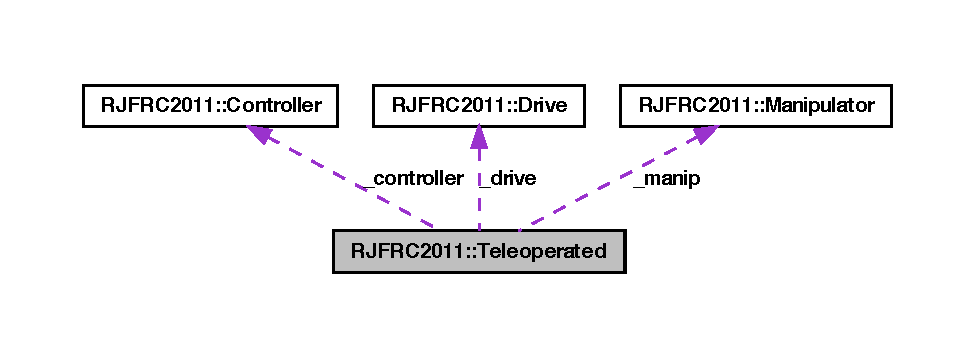
\includegraphics[width=400pt]{class_r_j_f_r_c2011_1_1_teleoperated__coll__graph}
\end{center}
\end{figure}
\subsection*{Public Member Functions}
\begin{DoxyCompactItemize}
\item 
\hyperlink{class_r_j_f_r_c2011_1_1_teleoperated_a4faee78835700892307b89c9977f523e}{Teleoperated} (\hyperlink{class_r_j_f_r_c2011_1_1_drive}{Drive} $\ast$drive, \hyperlink{class_r_j_f_r_c2011_1_1_manipulator}{Manipulator} $\ast$manip, \hyperlink{class_r_j_f_r_c2011_1_1_controller}{Controller} $\ast$controller, DriverStationLCD $\ast$screen)
\begin{DoxyCompactList}\small\item\em Construct from the addresses of a drive system, a manipulator, a controller, and the driver station LCD screen. \item\end{DoxyCompactList}\item 
\hypertarget{class_r_j_f_r_c2011_1_1_teleoperated_a19603fc214137c80b292de4ccf5fd3ec}{
\hyperlink{class_r_j_f_r_c2011_1_1_teleoperated_a19603fc214137c80b292de4ccf5fd3ec}{$\sim$Teleoperated} ()}
\label{class_r_j_f_r_c2011_1_1_teleoperated_a19603fc214137c80b292de4ccf5fd3ec}

\begin{DoxyCompactList}\small\item\em Destructor. Kill stuff. \item\end{DoxyCompactList}\item 
\hypertarget{class_r_j_f_r_c2011_1_1_teleoperated_a12d319115a887d3308c5f0a74d0df10f}{
void \hyperlink{class_r_j_f_r_c2011_1_1_teleoperated_a12d319115a887d3308c5f0a74d0df10f}{Init} ()}
\label{class_r_j_f_r_c2011_1_1_teleoperated_a12d319115a887d3308c5f0a74d0df10f}

\begin{DoxyCompactList}\small\item\em Set up for \hyperlink{class_r_j_f_r_c2011_1_1_teleoperated}{Teleoperated} mode. \item\end{DoxyCompactList}\item 
void \hyperlink{class_r_j_f_r_c2011_1_1_teleoperated_a22fa5b99fdf48c16e4f86db0bb0f4c02}{Go} ()
\begin{DoxyCompactList}\small\item\em This is where the magic happens. Get driver input, then figure out what to do with it. \item\end{DoxyCompactList}\item 
\hypertarget{class_r_j_f_r_c2011_1_1_teleoperated_a885303324836622da915a1204ac5e9bf}{
void \hyperlink{class_r_j_f_r_c2011_1_1_teleoperated_a885303324836622da915a1204ac5e9bf}{testLimitSwitches} ()}
\label{class_r_j_f_r_c2011_1_1_teleoperated_a885303324836622da915a1204ac5e9bf}

\begin{DoxyCompactList}\small\item\em Print the values we're getting from the limit switches to the screen. \item\end{DoxyCompactList}\end{DoxyCompactItemize}
\subsection*{Private Attributes}
\begin{DoxyCompactItemize}
\item 
\hypertarget{class_r_j_f_r_c2011_1_1_teleoperated_acf24bc9abe43a00df74559378f5eef09}{
\hyperlink{class_r_j_f_r_c2011_1_1_drive}{Drive} $\ast$ \hyperlink{class_r_j_f_r_c2011_1_1_teleoperated_acf24bc9abe43a00df74559378f5eef09}{\_\-drive}}
\label{class_r_j_f_r_c2011_1_1_teleoperated_acf24bc9abe43a00df74559378f5eef09}

\begin{DoxyCompactList}\small\item\em Pointer to object abstracting drive system. \item\end{DoxyCompactList}\item 
\hypertarget{class_r_j_f_r_c2011_1_1_teleoperated_a79579c70472b11af4938659c19c246a0}{
\hyperlink{class_r_j_f_r_c2011_1_1_manipulator}{Manipulator} $\ast$ \hyperlink{class_r_j_f_r_c2011_1_1_teleoperated_a79579c70472b11af4938659c19c246a0}{\_\-manip}}
\label{class_r_j_f_r_c2011_1_1_teleoperated_a79579c70472b11af4938659c19c246a0}

\begin{DoxyCompactList}\small\item\em Pointer to object abstracting manipulator. \item\end{DoxyCompactList}\item 
\hypertarget{class_r_j_f_r_c2011_1_1_teleoperated_a7ebf1a9b8ed5f9ac5174c524f50babc0}{
\hyperlink{class_r_j_f_r_c2011_1_1_controller}{Controller} $\ast$ \hyperlink{class_r_j_f_r_c2011_1_1_teleoperated_a7ebf1a9b8ed5f9ac5174c524f50babc0}{\_\-controller}}
\label{class_r_j_f_r_c2011_1_1_teleoperated_a7ebf1a9b8ed5f9ac5174c524f50babc0}

\begin{DoxyCompactList}\small\item\em Pointer to object abstracting controller. \item\end{DoxyCompactList}\item 
\hypertarget{class_r_j_f_r_c2011_1_1_teleoperated_a6a158c8efb6eb673ef4aceb89c614ba6}{
DriverStationLCD $\ast$ \hyperlink{class_r_j_f_r_c2011_1_1_teleoperated_a6a158c8efb6eb673ef4aceb89c614ba6}{\_\-screen}}
\label{class_r_j_f_r_c2011_1_1_teleoperated_a6a158c8efb6eb673ef4aceb89c614ba6}

\begin{DoxyCompactList}\small\item\em The screen of the driver station. \item\end{DoxyCompactList}\item 
\hypertarget{class_r_j_f_r_c2011_1_1_teleoperated_addd1786ca5cf7b7ddcccb2096aa2d934}{
Relay $\ast$ \hyperlink{class_r_j_f_r_c2011_1_1_teleoperated_addd1786ca5cf7b7ddcccb2096aa2d934}{minibotShelf}}
\label{class_r_j_f_r_c2011_1_1_teleoperated_addd1786ca5cf7b7ddcccb2096aa2d934}

\begin{DoxyCompactList}\small\item\em The minibot shelf relay. \item\end{DoxyCompactList}\item 
\hypertarget{class_r_j_f_r_c2011_1_1_teleoperated_abb83059ecad14dc769094bfabc77399d}{
DigitalInput $\ast$ \hyperlink{class_r_j_f_r_c2011_1_1_teleoperated_abb83059ecad14dc769094bfabc77399d}{top}}
\label{class_r_j_f_r_c2011_1_1_teleoperated_abb83059ecad14dc769094bfabc77399d}

\begin{DoxyCompactList}\small\item\em Top manipulator limit switch. \item\end{DoxyCompactList}\item 
\hypertarget{class_r_j_f_r_c2011_1_1_teleoperated_a3daa75d78f5d01924876ef42c99ca7a1}{
DigitalInput $\ast$ \hyperlink{class_r_j_f_r_c2011_1_1_teleoperated_a3daa75d78f5d01924876ef42c99ca7a1}{bottom}}
\label{class_r_j_f_r_c2011_1_1_teleoperated_a3daa75d78f5d01924876ef42c99ca7a1}

\begin{DoxyCompactList}\small\item\em Bottom manipulator limit switch. \item\end{DoxyCompactList}\item 
\hypertarget{class_r_j_f_r_c2011_1_1_teleoperated_ae73746c690998c02e4b5bd1912e83585}{
float \hyperlink{class_r_j_f_r_c2011_1_1_teleoperated_ae73746c690998c02e4b5bd1912e83585}{manipulatorElevation}}
\label{class_r_j_f_r_c2011_1_1_teleoperated_ae73746c690998c02e4b5bd1912e83585}

\begin{DoxyCompactList}\small\item\em User input: requested manipulator elevation. \item\end{DoxyCompactList}\item 
\hypertarget{class_r_j_f_r_c2011_1_1_teleoperated_af78f94699cab83d5936d4b783bf29ed7}{
float \hyperlink{class_r_j_f_r_c2011_1_1_teleoperated_af78f94699cab83d5936d4b783bf29ed7}{driveSpeed}}
\label{class_r_j_f_r_c2011_1_1_teleoperated_af78f94699cab83d5936d4b783bf29ed7}

\begin{DoxyCompactList}\small\item\em User input: requested drive speed. \item\end{DoxyCompactList}\item 
\hypertarget{class_r_j_f_r_c2011_1_1_teleoperated_ad2a716aacf9ab3d2379c0255bb193638}{
float \hyperlink{class_r_j_f_r_c2011_1_1_teleoperated_ad2a716aacf9ab3d2379c0255bb193638}{driveTurn}}
\label{class_r_j_f_r_c2011_1_1_teleoperated_ad2a716aacf9ab3d2379c0255bb193638}

\begin{DoxyCompactList}\small\item\em User input: requested drive turn. \item\end{DoxyCompactList}\item 
\hypertarget{class_r_j_f_r_c2011_1_1_teleoperated_a84e0dd4584d3c97475a0dde1242d485f}{
int \hyperlink{class_r_j_f_r_c2011_1_1_teleoperated_a84e0dd4584d3c97475a0dde1242d485f}{manipulatorAction}}
\label{class_r_j_f_r_c2011_1_1_teleoperated_a84e0dd4584d3c97475a0dde1242d485f}

\begin{DoxyCompactList}\small\item\em User input: requested manipulator action. \item\end{DoxyCompactList}\item 
\hypertarget{class_r_j_f_r_c2011_1_1_teleoperated_ae1d4ce201074832575f6a5dbe34a7c78}{
int \hyperlink{class_r_j_f_r_c2011_1_1_teleoperated_ae1d4ce201074832575f6a5dbe34a7c78}{minibotSwitches}}
\label{class_r_j_f_r_c2011_1_1_teleoperated_ae1d4ce201074832575f6a5dbe34a7c78}

\begin{DoxyCompactList}\small\item\em User input: requested minibot switches. \item\end{DoxyCompactList}\item 
\hypertarget{class_r_j_f_r_c2011_1_1_teleoperated_a8a3025d8bc20673eb7db70db765fa1ff}{
int \hyperlink{class_r_j_f_r_c2011_1_1_teleoperated_a8a3025d8bc20673eb7db70db765fa1ff}{\_\-nextState}}
\label{class_r_j_f_r_c2011_1_1_teleoperated_a8a3025d8bc20673eb7db70db765fa1ff}

\begin{DoxyCompactList}\small\item\em Used internally (in {\itshape genericCondition()\/}) to manage state switching. \item\end{DoxyCompactList}\item 
\hypertarget{class_r_j_f_r_c2011_1_1_teleoperated_a68b5dd3cb2442b6b722de3aa75e9dfee}{
bool \hyperlink{class_r_j_f_r_c2011_1_1_teleoperated_a68b5dd3cb2442b6b722de3aa75e9dfee}{rotateTubeDownFlag}}
\label{class_r_j_f_r_c2011_1_1_teleoperated_a68b5dd3cb2442b6b722de3aa75e9dfee}

\begin{DoxyCompactList}\small\item\em Used to flag that we want to rotate the tube down (after inputting it) \item\end{DoxyCompactList}\end{DoxyCompactItemize}


\subsection{Detailed Description}
Class managing robot performance in \hyperlink{class_r_j_f_r_c2011_1_1_teleoperated}{Teleoperated} mode. Gets user input from two controllers (abstracted as instances of class {\itshape Joystick\/}), processes said inputs (normalizing joystick values, dead space, etc.), and feeds them to a series of outputs (mainly the {\itshape \hyperlink{class_r_j_f_r_c2011_1_1_drive}{Drive}\/} class). 

\subsection{Constructor \& Destructor Documentation}
\hypertarget{class_r_j_f_r_c2011_1_1_teleoperated_a4faee78835700892307b89c9977f523e}{
\index{RJFRC2011::Teleoperated@{RJFRC2011::Teleoperated}!Teleoperated@{Teleoperated}}
\index{Teleoperated@{Teleoperated}!RJFRC2011::Teleoperated@{RJFRC2011::Teleoperated}}
\subsubsection[{Teleoperated}]{\setlength{\rightskip}{0pt plus 5cm}RJFRC2011::Teleoperated::Teleoperated (
\begin{DoxyParamCaption}
\item[{{\bf Drive} $\ast$}]{drive, }
\item[{{\bf Manipulator} $\ast$}]{manip, }
\item[{{\bf Controller} $\ast$}]{controller, }
\item[{DriverStationLCD $\ast$}]{screen}
\end{DoxyParamCaption}
)}}
\label{class_r_j_f_r_c2011_1_1_teleoperated_a4faee78835700892307b89c9977f523e}


Construct from the addresses of a drive system, a manipulator, a controller, and the driver station LCD screen. 

Set up pointers to passed adresses. Initialize state and condition pointers. 

\subsection{Member Function Documentation}
\hypertarget{class_r_j_f_r_c2011_1_1_teleoperated_a22fa5b99fdf48c16e4f86db0bb0f4c02}{
\index{RJFRC2011::Teleoperated@{RJFRC2011::Teleoperated}!Go@{Go}}
\index{Go@{Go}!RJFRC2011::Teleoperated@{RJFRC2011::Teleoperated}}
\subsubsection[{Go}]{\setlength{\rightskip}{0pt plus 5cm}void RJFRC2011::Teleoperated::Go (
\begin{DoxyParamCaption}
{}
\end{DoxyParamCaption}
)}}
\label{class_r_j_f_r_c2011_1_1_teleoperated_a22fa5b99fdf48c16e4f86db0bb0f4c02}


This is where the magic happens. Get driver input, then figure out what to do with it. 

Get input from the controller (see {\itshape \hyperlink{class_r_j_f_r_c2011_1_1_controller}{Controller}\/} class). Based on this, decide what values to send to the {\itshape \hyperlink{class_r_j_f_r_c2011_1_1_drive}{Drive}\/} class and {\itshape \hyperlink{class_r_j_f_r_c2011_1_1_manipulator}{Manipulator}\/} class, as well as how to move the relay ({\itshape Relay\/} class) controlling the minibot deployment system. 

The documentation for this class was generated from the following files:\begin{DoxyCompactItemize}
\item 
\hyperlink{_teleoperated_8h}{Teleoperated.h}\item 
\hyperlink{_teleoperated_8cpp}{Teleoperated.cpp}\end{DoxyCompactItemize}

\chapter{File Documentation}
\hypertarget{_autonomous_8cpp}{
\section{Autonomous.cpp File Reference}
\label{_autonomous_8cpp}\index{Autonomous.cpp@{Autonomous.cpp}}
}


File containing implementations of functions found in the {\itshape Autonomous\/} class (found in \hyperlink{_autonomous_8h}{Autonomous.h})  


{\ttfamily \#include \char`\"{}macros.h\char`\"{}}\par
{\ttfamily \#include \char`\"{}WPILib.h\char`\"{}}\par
{\ttfamily \#include \char`\"{}Autonomous.h\char`\"{}}\par
Include dependency graph for Autonomous.cpp:
\nopagebreak
\begin{figure}[H]
\begin{center}
\leavevmode
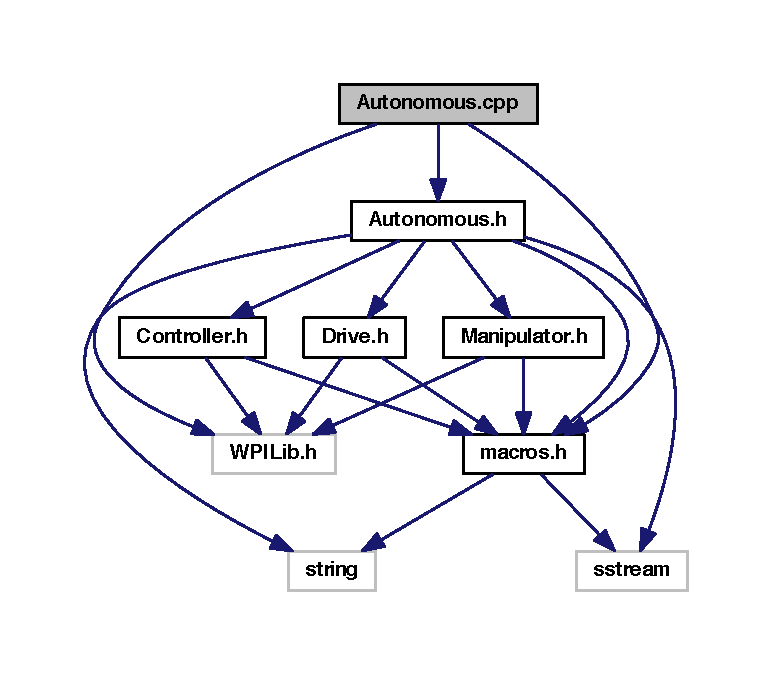
\includegraphics[width=368pt]{_autonomous_8cpp__incl}
\end{center}
\end{figure}


\subsection{Detailed Description}
File containing implementations of functions found in the {\itshape Autonomous\/} class (found in \hyperlink{_autonomous_8h}{Autonomous.h}) \begin{DoxyAuthor}{Authors}
Matthew Haney, Drew Lazzeri 
\end{DoxyAuthor}

\hypertarget{_autonomous_8h}{
\section{Autonomous.h File Reference}
\label{_autonomous_8h}\index{Autonomous.h@{Autonomous.h}}
}


File containing definition of {\itshape Autonomous\/} class, which is used within the {\itshape AutomonousPeriodic\/} function in the main program to simplify things.  


{\ttfamily \#include \char`\"{}macros.h\char`\"{}}\par
{\ttfamily \#include \char`\"{}Drive.h\char`\"{}}\par
{\ttfamily \#include \char`\"{}Manipulator.h\char`\"{}}\par
{\ttfamily \#include \char`\"{}Controller.h\char`\"{}}\par
{\ttfamily \#include $<$string$>$}\par
{\ttfamily \#include $<$sstream$>$}\par
Include dependency graph for Autonomous.h:\nopagebreak
\begin{figure}[H]
\begin{center}
\leavevmode
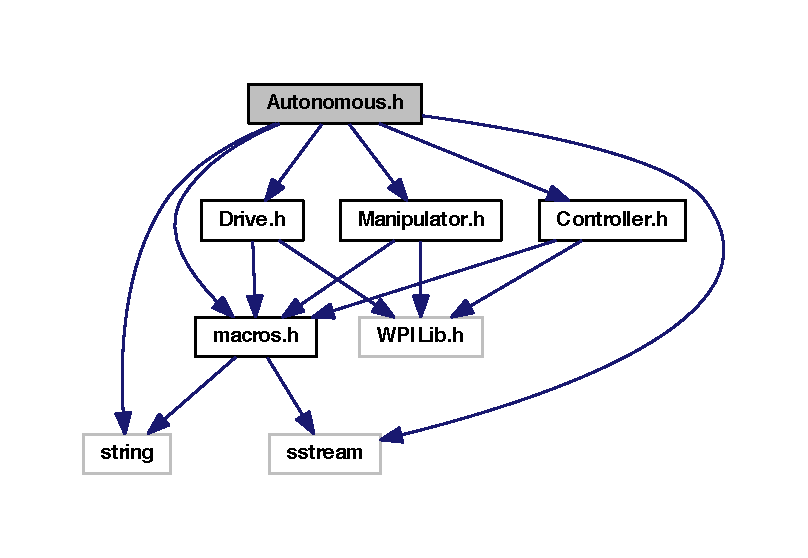
\includegraphics[width=385pt]{_autonomous_8h__incl}
\end{center}
\end{figure}
This graph shows which files directly or indirectly include this file:\nopagebreak
\begin{figure}[H]
\begin{center}
\leavevmode
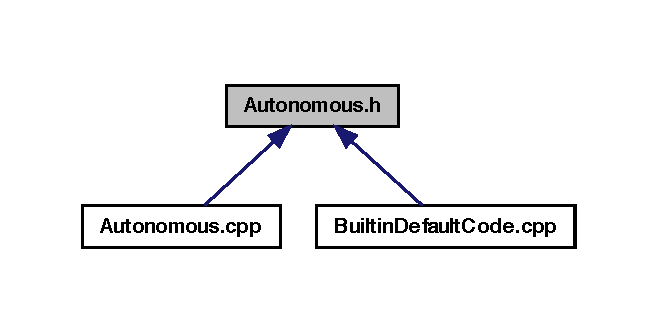
\includegraphics[width=316pt]{_autonomous_8h__dep__incl}
\end{center}
\end{figure}
\subsection*{Classes}
\begin{DoxyCompactItemize}
\item 
class \hyperlink{class_r_j_f_r_c2011_1_1_autonomous}{RJFRC2011::Autonomous}
\begin{DoxyCompactList}\small\item\em Class managing the \hyperlink{class_r_j_f_r_c2011_1_1_autonomous}{Autonomous} period of the competition. \item\end{DoxyCompactList}\end{DoxyCompactItemize}


\subsection{Detailed Description}
File containing definition of {\itshape Autonomous\/} class, which is used within the {\itshape AutomonousPeriodic\/} function in the main program to simplify things. \begin{DoxyAuthor}{Authors}
Matthew Haney, Drew Lazzeri 
\end{DoxyAuthor}

\hypertarget{_axis_camera_8cpp}{
\section{AxisCamera.cpp File Reference}
\label{_axis_camera_8cpp}\index{AxisCamera.cpp@{AxisCamera.cpp}}
}


File patching buggy code for the AxisCamera class that causes the robot to freeze.  


{\ttfamily \#include $<$string.h$>$}\par
{\ttfamily \#include \char`\"{}Synchronized.h\char`\"{}}\par
{\ttfamily \#include \char`\"{}Vision/AxisCamera.h\char`\"{}}\par
{\ttfamily \#include \char`\"{}Vision/PCVideoServer.h\char`\"{}}\par
Include dependency graph for AxisCamera.cpp:
\nopagebreak
\begin{figure}[H]
\begin{center}
\leavevmode
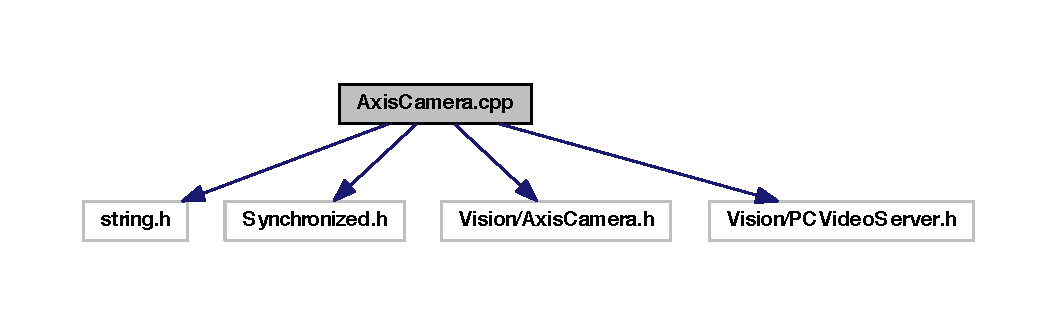
\includegraphics[width=400pt]{_axis_camera_8cpp__incl}
\end{center}
\end{figure}


\subsection{Detailed Description}
File patching buggy code for the AxisCamera class that causes the robot to freeze. \begin{DoxyAuthor}{Authors}
FIRST people, Joe Hurler 
\end{DoxyAuthor}

\hypertarget{_axis_camera_params_8cpp}{
\section{AxisCameraParams.cpp File Reference}
\label{_axis_camera_params_8cpp}\index{AxisCameraParams.cpp@{AxisCameraParams.cpp}}
}


File patching buggy code for the AxisCameraParams class that causes the robot to freeze. All documentation included was provided by Hurler and/or FIRST, though it was reformatted to be compatible with Doxygen.  


{\ttfamily \#include \char`\"{}Vision/AxisCameraParams.h\char`\"{}}\par
{\ttfamily \#include \char`\"{}Vision/AxisCamera.h\char`\"{}}\par
{\ttfamily \#include $<$inetLib.h$>$}\par
{\ttfamily \#include \char`\"{}pcre.h\char`\"{}}\par
{\ttfamily \#include $<$sockLib.h$>$}\par
{\ttfamily \#include $<$string.h$>$}\par
{\ttfamily \#include \char`\"{}Synchronized.h\char`\"{}}\par
{\ttfamily \#include \char`\"{}Timer.h\char`\"{}}\par
Include dependency graph for AxisCameraParams.cpp:\nopagebreak
\begin{figure}[H]
\begin{center}
\leavevmode
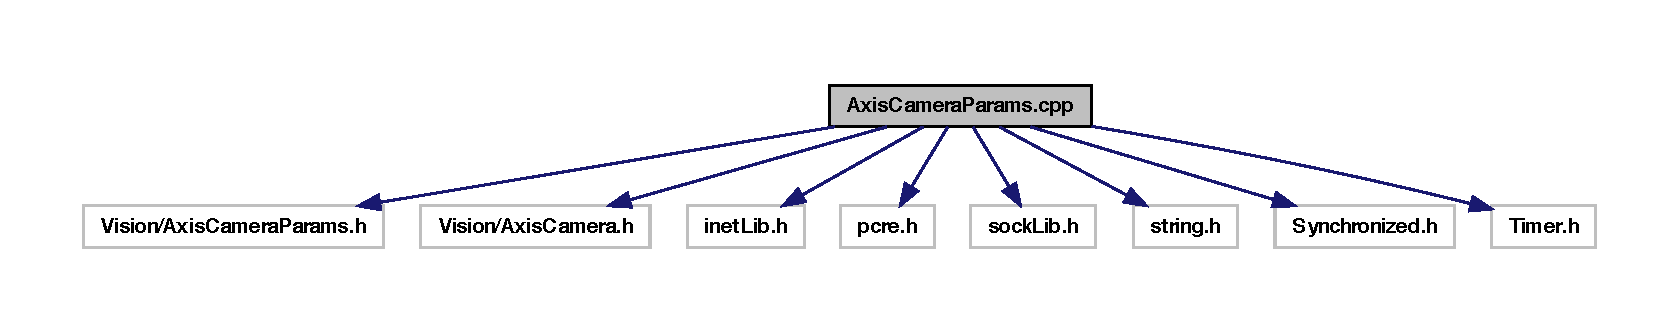
\includegraphics[width=400pt]{_axis_camera_params_8cpp__incl}
\end{center}
\end{figure}


\subsection{Detailed Description}
File patching buggy code for the AxisCameraParams class that causes the robot to freeze. All documentation included was provided by Hurler and/or FIRST, though it was reformatted to be compatible with Doxygen. \begin{DoxyAuthor}{Authors}
FIRST people, Joe Hurler 
\end{DoxyAuthor}

\hypertarget{_builtin_default_code_8cpp}{
\section{BuiltinDefaultCode.cpp File Reference}
\label{_builtin_default_code_8cpp}\index{BuiltinDefaultCode.cpp@{BuiltinDefaultCode.cpp}}
}


The file containing the class \hyperlink{class_builtin_default_code}{BuiltinDefaultCode}. We didn't bother changing the name...  


{\ttfamily \#include \char`\"{}macros.h\char`\"{}}\par
{\ttfamily \#include \char`\"{}WPILib.h\char`\"{}}\par
{\ttfamily \#include \char`\"{}Autonomous.h\char`\"{}}\par
{\ttfamily \#include \char`\"{}Teleoperated.h\char`\"{}}\par
{\ttfamily \#include \char`\"{}Controller.h\char`\"{}}\par
{\ttfamily \#include $<$sstream$>$}\par
\subsection*{Classes}
\begin{DoxyCompactItemize}
\item 
class \hyperlink{class_builtin_default_code}{BuiltinDefaultCode}
\begin{DoxyCompactList}\small\item\em Our big class that does everything. We didn't bother renaming it. \item\end{DoxyCompactList}\end{DoxyCompactItemize}


\subsection{Detailed Description}
The file containing the class \hyperlink{class_builtin_default_code}{BuiltinDefaultCode}. We didn't bother changing the name... The main source code file for Regis Jesuit High School FRC Team \#3729. \begin{DoxyAuthor}{Authors}
Matthew Haney, Drew Lazzerri 
\end{DoxyAuthor}

\hypertarget{_controller_8cpp}{
\section{Controller.cpp File Reference}
\label{_controller_8cpp}\index{Controller.cpp@{Controller.cpp}}
}


File containing implementations of functions found in the {\itshape Controller\/} class (found in \hyperlink{_controller_8h}{Controller.h})  


{\ttfamily \#include \char`\"{}Controller.h\char`\"{}}\par
{\ttfamily \#include \char`\"{}WPILib.h\char`\"{}}\par
{\ttfamily \#include \char`\"{}macros.h\char`\"{}}\par
Include dependency graph for Controller.cpp:
\nopagebreak
\begin{figure}[H]
\begin{center}
\leavevmode
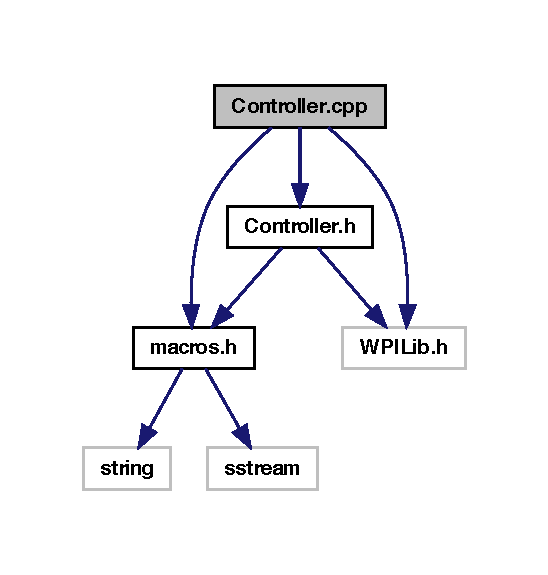
\includegraphics[width=263pt]{_controller_8cpp__incl}
\end{center}
\end{figure}


\subsection{Detailed Description}
File containing implementations of functions found in the {\itshape Controller\/} class (found in \hyperlink{_controller_8h}{Controller.h}) \begin{DoxyAuthor}{Authors}
Matthew Haney, Drew Lazzeri 
\end{DoxyAuthor}

\hypertarget{_controller_8h}{
\section{Controller.h File Reference}
\label{_controller_8h}\index{Controller.h@{Controller.h}}
}


File containing definition of {\itshape Controller\/} class, which is used in both Autonomous and Teleoperated modes to get user input.  


{\ttfamily \#include \char`\"{}macros.h\char`\"{}}\par
{\ttfamily \#include \char`\"{}WPILib.h\char`\"{}}\par
Include dependency graph for Controller.h:\nopagebreak
\begin{figure}[H]
\begin{center}
\leavevmode
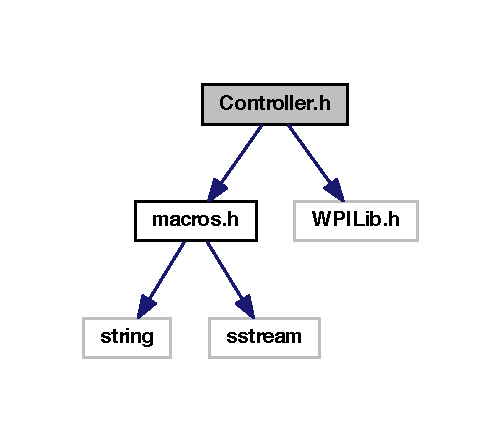
\includegraphics[width=238pt]{_controller_8h__incl}
\end{center}
\end{figure}
This graph shows which files directly or indirectly include this file:\nopagebreak
\begin{figure}[H]
\begin{center}
\leavevmode
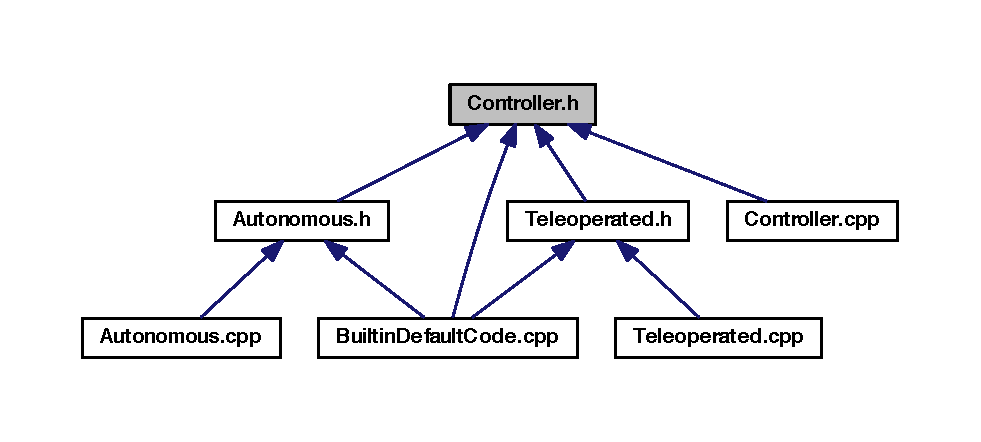
\includegraphics[width=400pt]{_controller_8h__dep__incl}
\end{center}
\end{figure}
\subsection*{Classes}
\begin{DoxyCompactItemize}
\item 
class \hyperlink{class_r_j_f_r_c2011_1_1_controller}{RJFRC2011::Controller}
\begin{DoxyCompactList}\small\item\em Class abstracting the controller(s) used by our driver(s) \item\end{DoxyCompactList}\end{DoxyCompactItemize}


\subsection{Detailed Description}
File containing definition of {\itshape Controller\/} class, which is used in both Autonomous and Teleoperated modes to get user input. \begin{DoxyAuthor}{Authors}
Matthew Haney, Drew Lazzeri 
\end{DoxyAuthor}

\hypertarget{_drive_8cpp}{
\section{Drive.cpp File Reference}
\label{_drive_8cpp}\index{Drive.cpp@{Drive.cpp}}
}


File containing definitions of functions declared in class {\itshape Drive\/} (declared in \hyperlink{_drive_8h}{Drive.h}).  


{\ttfamily \#include \char`\"{}Drive.h\char`\"{}}\par
{\ttfamily \#include \char`\"{}WPILib.h\char`\"{}}\par
Include dependency graph for Drive.cpp:\nopagebreak
\begin{figure}[H]
\begin{center}
\leavevmode
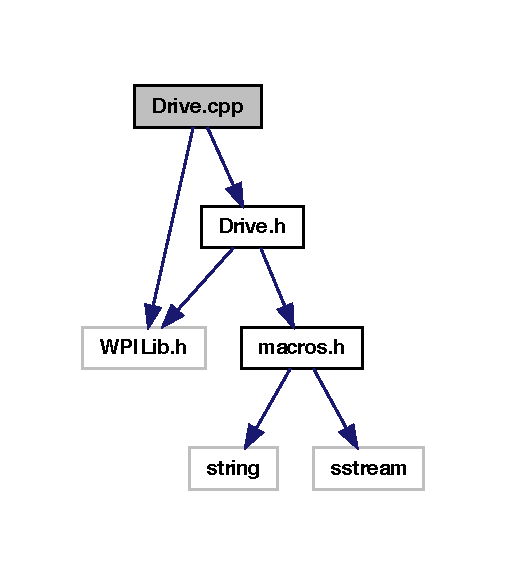
\includegraphics[width=243pt]{_drive_8cpp__incl}
\end{center}
\end{figure}


\subsection{Detailed Description}
File containing definitions of functions declared in class {\itshape Drive\/} (declared in \hyperlink{_drive_8h}{Drive.h}). 
\hypertarget{_drive_8h}{
\section{Drive.h File Reference}
\label{_drive_8h}\index{Drive.h@{Drive.h}}
}


File containing definition of {\itshape Drive\/} class, which is used in the main program to drive the robot in both Autonomous and Teleoperated modes with no waste of memory.  


{\ttfamily \#include \char`\"{}WPILib.h\char`\"{}}\par
{\ttfamily \#include \char`\"{}macros.h\char`\"{}}\par
Include dependency graph for Drive.h:
\nopagebreak
\begin{figure}[H]
\begin{center}
\leavevmode
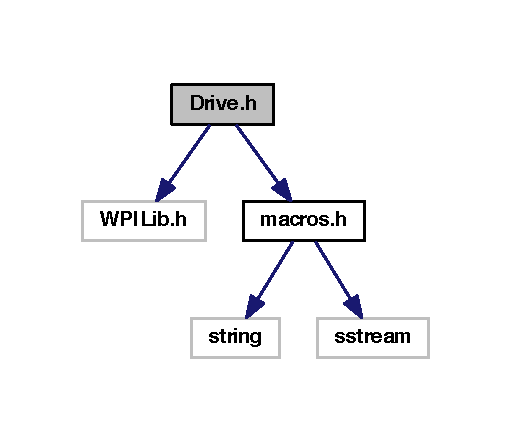
\includegraphics[width=243pt]{_drive_8h__incl}
\end{center}
\end{figure}
This graph shows which files directly or indirectly include this file:
\nopagebreak
\begin{figure}[H]
\begin{center}
\leavevmode
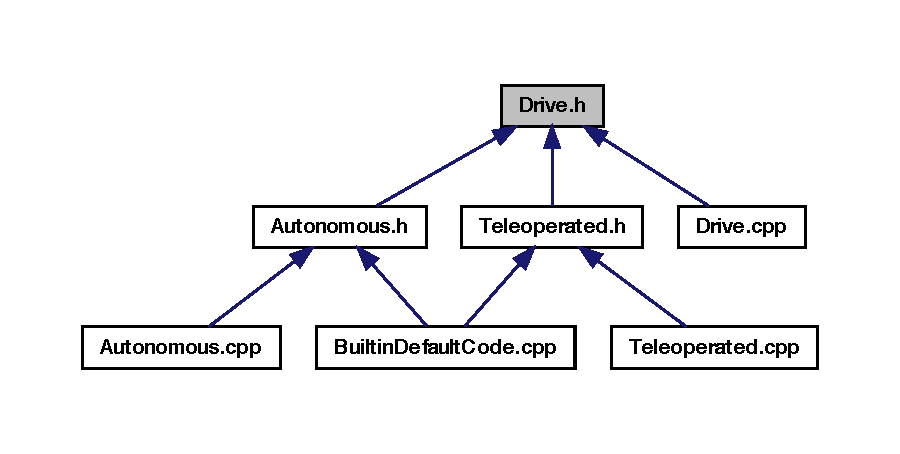
\includegraphics[width=400pt]{_drive_8h__dep__incl}
\end{center}
\end{figure}
\subsection*{Classes}
\begin{DoxyCompactItemize}
\item 
class \hyperlink{class_r_j_f_r_c2011_1_1_drive}{RJFRC2011::Drive}
\begin{DoxyCompactList}\small\item\em Class abstracting the drive system. \item\end{DoxyCompactList}\end{DoxyCompactItemize}


\subsection{Detailed Description}
File containing definition of {\itshape Drive\/} class, which is used in the main program to drive the robot in both Autonomous and Teleoperated modes with no waste of memory. \begin{DoxyAuthor}{Authors}
Matthew Haney, Drew Lazzeri 
\end{DoxyAuthor}

\hypertarget{macros_8h}{
\section{macros.h File Reference}
\label{macros_8h}\index{macros.h@{macros.h}}
}


File containing a bunch of macros to de-\/clutter our other files.  


{\ttfamily \#include $<$string$>$}\par
{\ttfamily \#include $<$sstream$>$}\par
\subsection*{Defines}
\begin{DoxyCompactItemize}
\item 
\hypertarget{macros_8h_a244c5fd1d94aa1f4f4b65d3c79d9c72c}{
\#define \hyperlink{macros_8h_a244c5fd1d94aa1f4f4b65d3c79d9c72c}{YCENTER}~(0.03125)}
\label{macros_8h_a244c5fd1d94aa1f4f4b65d3c79d9c72c}

\begin{DoxyCompactList}\small\item\em Adjustment for the fact that the joystick is slightly off-\/center. \item\end{DoxyCompactList}\item 
\hypertarget{macros_8h_a127f99ac79d5012d50317daf88e7f1a6}{
\#define \hyperlink{macros_8h_a127f99ac79d5012d50317daf88e7f1a6}{ROTCENTER}~(0.0156)}
\label{macros_8h_a127f99ac79d5012d50317daf88e7f1a6}

\begin{DoxyCompactList}\small\item\em Adjustment for the fact that the joystick is slightly off-\/center. \item\end{DoxyCompactList}\item 
\hypertarget{macros_8h_a6aee779504f876f9bed834f36b392da9}{
\#define \hyperlink{macros_8h_a6aee779504f876f9bed834f36b392da9}{XMIN}~-\/0.641}
\label{macros_8h_a6aee779504f876f9bed834f36b392da9}

\begin{DoxyCompactList}\small\item\em Minimum possible X value. \item\end{DoxyCompactList}\item 
\hypertarget{macros_8h_a0312cb6d6cbc719075d4e5380c387ab3}{
\#define \hyperlink{macros_8h_a0312cb6d6cbc719075d4e5380c387ab3}{XMAX}~0.648}
\label{macros_8h_a0312cb6d6cbc719075d4e5380c387ab3}

\begin{DoxyCompactList}\small\item\em Maximum possible X value. \item\end{DoxyCompactList}\item 
\hypertarget{macros_8h_aa025181dff552575490c5148a493ff65}{
\#define \hyperlink{macros_8h_aa025181dff552575490c5148a493ff65}{YMIN}~(-\/0.57-\/YCENTER)}
\label{macros_8h_aa025181dff552575490c5148a493ff65}

\begin{DoxyCompactList}\small\item\em Minimum possible Y value. \item\end{DoxyCompactList}\item 
\hypertarget{macros_8h_a610d6ad95b18966b70b6845de2a9c56b}{
\#define \hyperlink{macros_8h_a610d6ad95b18966b70b6845de2a9c56b}{YMAX}~(0.641-\/YCENTER)}
\label{macros_8h_a610d6ad95b18966b70b6845de2a9c56b}

\begin{DoxyCompactList}\small\item\em Maximum possilble Y value. \item\end{DoxyCompactList}\item 
\hypertarget{macros_8h_aea4c8e7fa16752c56ffad3be5e533de5}{
\#define \hyperlink{macros_8h_aea4c8e7fa16752c56ffad3be5e533de5}{ZMIN}~(-\/0.54)}
\label{macros_8h_aea4c8e7fa16752c56ffad3be5e533de5}

\begin{DoxyCompactList}\small\item\em Minimum possible Z value. \item\end{DoxyCompactList}\item 
\hypertarget{macros_8h_a131010b0d7e64a592f782aec28c6a4d8}{
\#define \hyperlink{macros_8h_a131010b0d7e64a592f782aec28c6a4d8}{ZMAX}~(0.63)}
\label{macros_8h_a131010b0d7e64a592f782aec28c6a4d8}

\begin{DoxyCompactList}\small\item\em Maximum possible Z value. \item\end{DoxyCompactList}\item 
\hypertarget{macros_8h_ad105605859fafc75c6093a346292aa19}{
\#define \hyperlink{macros_8h_ad105605859fafc75c6093a346292aa19}{ROTMIN}~(-\/0.64-\/ROTCENTER)}
\label{macros_8h_ad105605859fafc75c6093a346292aa19}

\begin{DoxyCompactList}\small\item\em Minimum possible rotation value. \item\end{DoxyCompactList}\item 
\hypertarget{macros_8h_a2b7548b633da844f977399a2fd77ef24}{
\#define \hyperlink{macros_8h_a2b7548b633da844f977399a2fd77ef24}{ROTMAX}~(0.68-\/ROTCENTER)}
\label{macros_8h_a2b7548b633da844f977399a2fd77ef24}

\begin{DoxyCompactList}\small\item\em Maximum possible rotation value. \item\end{DoxyCompactList}\item 
\hypertarget{macros_8h_abca3e52dd0360248580f75b2280f7df0}{
\#define \hyperlink{macros_8h_abca3e52dd0360248580f75b2280f7df0}{XEXPO}~0.4}
\label{macros_8h_abca3e52dd0360248580f75b2280f7df0}

\begin{DoxyCompactList}\small\item\em Exponential constant for modifying input from the x-\/axis. \item\end{DoxyCompactList}\item 
\hypertarget{macros_8h_a58fb3136b9073b46d4f23aa16e5d14ce}{
\#define \hyperlink{macros_8h_a58fb3136b9073b46d4f23aa16e5d14ce}{YEXPO}~0.4}
\label{macros_8h_a58fb3136b9073b46d4f23aa16e5d14ce}

\begin{DoxyCompactList}\small\item\em Exponential constant for modfying input from the y-\/axis. \item\end{DoxyCompactList}\item 
\hypertarget{macros_8h_a464292d5bd5af44d16fc1049b775f434}{
\#define \hyperlink{macros_8h_a464292d5bd5af44d16fc1049b775f434}{ROTEXPO}~0.6}
\label{macros_8h_a464292d5bd5af44d16fc1049b775f434}

\begin{DoxyCompactList}\small\item\em Exponential constant for modifying input form the rotational axis. \item\end{DoxyCompactList}\item 
\hypertarget{macros_8h_af5c294bdd73073d40b59b5fb680da1f5}{
\#define \hyperlink{macros_8h_af5c294bdd73073d40b59b5fb680da1f5}{AUTONOMOUS\_\-LANE\_\-SWITCH\_\-PORT}~6}
\label{macros_8h_af5c294bdd73073d40b59b5fb680da1f5}

\begin{DoxyCompactList}\small\item\em Port \# for the physical lane choosing switch in Autonomous. \item\end{DoxyCompactList}\item 
\hypertarget{macros_8h_ad7ded68c32af86b724dfafe66b920ce9}{
\#define \hyperlink{macros_8h_ad7ded68c32af86b724dfafe66b920ce9}{AUTONOMOUS\_\-FORK\_\-SWITCH\_\-PORT}~7}
\label{macros_8h_ad7ded68c32af86b724dfafe66b920ce9}

\begin{DoxyCompactList}\small\item\em Port \# for the physical fork choosing switch in Autonomous. \item\end{DoxyCompactList}\item 
\hypertarget{macros_8h_a2c9350fc206ba58641929e083648be11}{
\#define \hyperlink{macros_8h_a2c9350fc206ba58641929e083648be11}{MANIPULATOR\_\-ELEVATION\_\-TOP\_\-LIMIT\_\-SWITCH\_\-PORT}~4}
\label{macros_8h_a2c9350fc206ba58641929e083648be11}

\begin{DoxyCompactList}\small\item\em Port \# for the limit switch at the top of the manipulator elevator's reach. \item\end{DoxyCompactList}\item 
\hypertarget{macros_8h_a5e22437986eee9a1fe8f44cf98b32483}{
\#define \hyperlink{macros_8h_a5e22437986eee9a1fe8f44cf98b32483}{MANIPULATOR\_\-ELEVATION\_\-BOTTOM\_\-LIMIT\_\-SWITCH\_\-PORT}~5}
\label{macros_8h_a5e22437986eee9a1fe8f44cf98b32483}

\begin{DoxyCompactList}\small\item\em Port \# for the limit switch at the bottom of the manipulator elevator's reach. \item\end{DoxyCompactList}\item 
\hypertarget{macros_8h_a4bc5e8af53eacd86a8333b2f148b7445}{
\#define \hyperlink{macros_8h_a4bc5e8af53eacd86a8333b2f148b7445}{LIGHT\_\-SENSOR\_\-LEFT\_\-PORT}~1}
\label{macros_8h_a4bc5e8af53eacd86a8333b2f148b7445}

\begin{DoxyCompactList}\small\item\em Port \# of the leftmost line-\/following light sensor. \item\end{DoxyCompactList}\item 
\hypertarget{macros_8h_a94797b3ebdf03143368647b3581de19d}{
\#define \hyperlink{macros_8h_a94797b3ebdf03143368647b3581de19d}{LIGHT\_\-SENSOR\_\-CENTER\_\-PORT}~2}
\label{macros_8h_a94797b3ebdf03143368647b3581de19d}

\begin{DoxyCompactList}\small\item\em Port \# of the center line-\/following light sensor. \item\end{DoxyCompactList}\item 
\hypertarget{macros_8h_a25d468051abadf3dfbed13ffab7a4833}{
\#define \hyperlink{macros_8h_a25d468051abadf3dfbed13ffab7a4833}{LIGHT\_\-SENSOR\_\-RIGHT\_\-PORT}~3}
\label{macros_8h_a25d468051abadf3dfbed13ffab7a4833}

\begin{DoxyCompactList}\small\item\em Port \# of the rightmost line-\/following light sensor. \item\end{DoxyCompactList}\item 
\hypertarget{macros_8h_ad7f9276864c8d3024ac469978baf1f05}{
\#define \hyperlink{macros_8h_ad7f9276864c8d3024ac469978baf1f05}{MINIBOT\_\-SHELF\_\-RELAY\_\-PORT}~1}
\label{macros_8h_ad7f9276864c8d3024ac469978baf1f05}

\begin{DoxyCompactList}\small\item\em Port \# for the relay controlling the minbot shelf. \item\end{DoxyCompactList}\item 
\hypertarget{macros_8h_ac1b9b0f3b1b26567061f78a109415cd2}{
\#define \hyperlink{macros_8h_ac1b9b0f3b1b26567061f78a109415cd2}{MANIPULATOR\_\-TOP\_\-RELAY\_\-PORT}~2}
\label{macros_8h_ac1b9b0f3b1b26567061f78a109415cd2}

\begin{DoxyCompactList}\small\item\em Port \# for the relay controlling the top wheels of the manipulator. \item\end{DoxyCompactList}\item 
\hypertarget{macros_8h_a001642e6e62eedc685167a8bdc5cfccd}{
\#define \hyperlink{macros_8h_a001642e6e62eedc685167a8bdc5cfccd}{MANIPULATOR\_\-BOTTOM\_\-RELAY\_\-PORT}~3}
\label{macros_8h_a001642e6e62eedc685167a8bdc5cfccd}

\begin{DoxyCompactList}\small\item\em Port \# for the relay controlling the bottom wheels of the manipulator. \item\end{DoxyCompactList}\item 
\hypertarget{macros_8h_a5982744ec70c5708a0a66ed629cf526d}{
\#define \hyperlink{macros_8h_a5982744ec70c5708a0a66ed629cf526d}{MANIPULATOR\_\-ELEVATION\_\-RELAY\_\-PORT}~4}
\label{macros_8h_a5982744ec70c5708a0a66ed629cf526d}

\begin{DoxyCompactList}\small\item\em Port \# for the relay controlling elevation of the manipulator. \item\end{DoxyCompactList}\item 
\hypertarget{macros_8h_aa5f262ae81a4bc71833be5df15b49ec1}{
\#define \hyperlink{macros_8h_aa5f262ae81a4bc71833be5df15b49ec1}{DRIVE\_\-FRONT\_\-LEFT\_\-JAGUAR\_\-PORT}~5}
\label{macros_8h_aa5f262ae81a4bc71833be5df15b49ec1}

\begin{DoxyCompactList}\small\item\em Port \# of the front left Jaguar on the drive train. \item\end{DoxyCompactList}\item 
\hypertarget{macros_8h_aa1d31f972d08b33df2300a0434ecedf7}{
\#define \hyperlink{macros_8h_aa1d31f972d08b33df2300a0434ecedf7}{DRIVE\_\-FRONT\_\-RIGHT\_\-JAGUAR\_\-PORT}~7}
\label{macros_8h_aa1d31f972d08b33df2300a0434ecedf7}

\begin{DoxyCompactList}\small\item\em Port \# of the front right Jaguar on the drive train. \item\end{DoxyCompactList}\item 
\hypertarget{macros_8h_a7e31d84902c3f5a88dfe615bb3d7d365}{
\#define \hyperlink{macros_8h_a7e31d84902c3f5a88dfe615bb3d7d365}{DRIVE\_\-BACK\_\-LEFT\_\-JAGUAR\_\-PORT}~6}
\label{macros_8h_a7e31d84902c3f5a88dfe615bb3d7d365}

\begin{DoxyCompactList}\small\item\em Port \# of the back left Jaguar on the drive train. \item\end{DoxyCompactList}\item 
\hypertarget{macros_8h_a66215ddced4940c9de38365d6a839841}{
\#define \hyperlink{macros_8h_a66215ddced4940c9de38365d6a839841}{DRIVE\_\-BACK\_\-RIGHT\_\-JAGUAR\_\-PORT}~8}
\label{macros_8h_a66215ddced4940c9de38365d6a839841}

\begin{DoxyCompactList}\small\item\em Port \# of the back right Jaguar on the drive train. \item\end{DoxyCompactList}\item 
\hypertarget{macros_8h_a35dd9359c9b8461811401247cd10753b}{
\#define \hyperlink{macros_8h_a35dd9359c9b8461811401247cd10753b}{DEFAULT\_\-WATCHDOG\_\-TIME}~3.0}
\label{macros_8h_a35dd9359c9b8461811401247cd10753b}

\begin{DoxyCompactList}\small\item\em The default expiration time of the Watchdog timer, in seconds. \item\end{DoxyCompactList}\item 
\hypertarget{macros_8h_ae746c51c6037381961c9313e8b62529c}{
\#define \hyperlink{macros_8h_ae746c51c6037381961c9313e8b62529c}{AUTO\_\-DRIVE\_\-SPEED}~0.35}
\label{macros_8h_ae746c51c6037381961c9313e8b62529c}

\begin{DoxyCompactList}\small\item\em Speed at which we drive in Autonomous. \item\end{DoxyCompactList}\item 
\hypertarget{macros_8h_aba3f3add9147af90e29a0d50ba3d16e8}{
\#define \hyperlink{macros_8h_aba3f3add9147af90e29a0d50ba3d16e8}{AUTO\_\-TURN\_\-SPEED}~0.65}
\label{macros_8h_aba3f3add9147af90e29a0d50ba3d16e8}

\begin{DoxyCompactList}\small\item\em Speed at which we turn in Autonomous. \item\end{DoxyCompactList}\item 
\hypertarget{macros_8h_af4d4038d993d1f32b9cae705ed987fbf}{
\#define \hyperlink{macros_8h_af4d4038d993d1f32b9cae705ed987fbf}{AUTO\_\-BRAKE\_\-SPEED}~-\/0.6}
\label{macros_8h_af4d4038d993d1f32b9cae705ed987fbf}

\begin{DoxyCompactList}\small\item\em Speed at which we brake in Autonomous. \item\end{DoxyCompactList}\end{DoxyCompactItemize}
\subsection*{Functions}
\begin{DoxyCompactItemize}
\item 
{\footnotesize template$<$typename T $>$ }\\const char $\ast$ \hyperlink{macros_8h_a70a742af36a2c566aee2804be7ae2ec4}{topchar} (T val)
\begin{DoxyCompactList}\small\item\em Convert an arbitrary type to a printable string, since this isn't Python. \item\end{DoxyCompactList}\end{DoxyCompactItemize}


\subsection{Detailed Description}
File containing a bunch of macros to de-\/clutter our other files. NOTE: All adjustment macros experimentally made by Adam Bryant. 

\subsection{Function Documentation}
\hypertarget{macros_8h_a70a742af36a2c566aee2804be7ae2ec4}{
\index{macros.h@{macros.h}!topchar@{topchar}}
\index{topchar@{topchar}!macros.h@{macros.h}}
\subsubsection[{topchar}]{\setlength{\rightskip}{0pt plus 5cm}template$<$typename T $>$ const char$\ast$ topchar (
\begin{DoxyParamCaption}
\item[{T}]{val}
\end{DoxyParamCaption}
)}}
\label{macros_8h_a70a742af36a2c566aee2804be7ae2ec4}


Convert an arbitrary type to a printable string, since this isn't Python. 


\begin{DoxyParams}{Parameters}
{\em val} & The number to be converted \\
\hline
\end{DoxyParams}
\begin{DoxyReturn}{Returns}
The string representation of the passed number 
\end{DoxyReturn}

\hypertarget{_manipulator_8cpp}{
\section{Manipulator.cpp File Reference}
\label{_manipulator_8cpp}\index{Manipulator.cpp@{Manipulator.cpp}}
}


File containing implementations of functions found in the {\itshape Manipulator\/} class (found in \hyperlink{_manipulator_8h}{Manipulator.h}).  


{\ttfamily \#include \char`\"{}Manipulator.h\char`\"{}}\par
{\ttfamily \#include \char`\"{}WPILib.h\char`\"{}}\par
{\ttfamily \#include \char`\"{}macros.h\char`\"{}}\par
Include dependency graph for Manipulator.cpp:\nopagebreak
\begin{figure}[H]
\begin{center}
\leavevmode
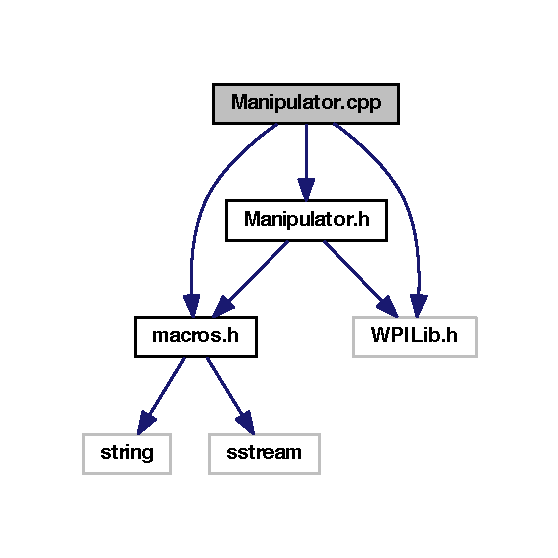
\includegraphics[width=266pt]{_manipulator_8cpp__incl}
\end{center}
\end{figure}


\subsection{Detailed Description}
File containing implementations of functions found in the {\itshape Manipulator\/} class (found in \hyperlink{_manipulator_8h}{Manipulator.h}). \begin{DoxyAuthor}{Authors}
Matthew Haney, Drew Lazzeri 
\end{DoxyAuthor}

\hypertarget{_manipulator_8h}{
\section{Manipulator.h File Reference}
\label{_manipulator_8h}\index{Manipulator.h@{Manipulator.h}}
}


File containing definition of {\itshape Manipulator\/} class, which is used to simulate the manipulator in both Autonomous and Periodic modes.  


{\ttfamily \#include \char`\"{}macros.h\char`\"{}}\par
{\ttfamily \#include \char`\"{}WPILib.h\char`\"{}}\par
Include dependency graph for Manipulator.h:
\nopagebreak
\begin{figure}[H]
\begin{center}
\leavevmode
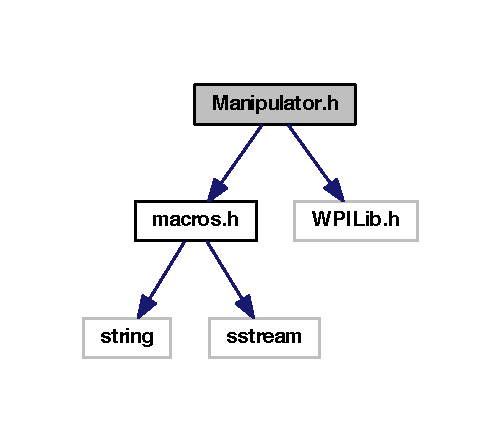
\includegraphics[width=238pt]{_manipulator_8h__incl}
\end{center}
\end{figure}
This graph shows which files directly or indirectly include this file:
\nopagebreak
\begin{figure}[H]
\begin{center}
\leavevmode
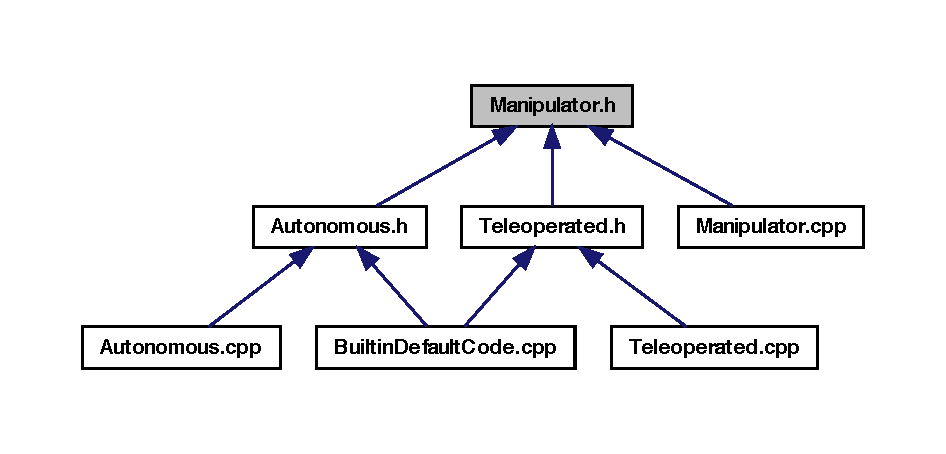
\includegraphics[width=400pt]{_manipulator_8h__dep__incl}
\end{center}
\end{figure}
\subsection*{Classes}
\begin{DoxyCompactItemize}
\item 
class \hyperlink{class_r_j_f_r_c2011_1_1_manipulator}{RJFRC2011::Manipulator}
\begin{DoxyCompactList}\small\item\em Abstracts the manipulator. \item\end{DoxyCompactList}\end{DoxyCompactItemize}


\subsection{Detailed Description}
File containing definition of {\itshape Manipulator\/} class, which is used to simulate the manipulator in both Autonomous and Periodic modes. \begin{DoxyAuthor}{Authors}
Matthew Haney, Drew Lazzeri 
\end{DoxyAuthor}

\hypertarget{_teleoperated_8cpp}{
\section{Teleoperated.cpp File Reference}
\label{_teleoperated_8cpp}\index{Teleoperated.cpp@{Teleoperated.cpp}}
}


File containing definitions of functions declared in class {\itshape Teleoperated\/} (declared in \hyperlink{_teleoperated_8h}{Teleoperated.h}).  


{\ttfamily \#include \char`\"{}Teleoperated.h\char`\"{}}\par
Include dependency graph for Teleoperated.cpp:\nopagebreak
\begin{figure}[H]
\begin{center}
\leavevmode
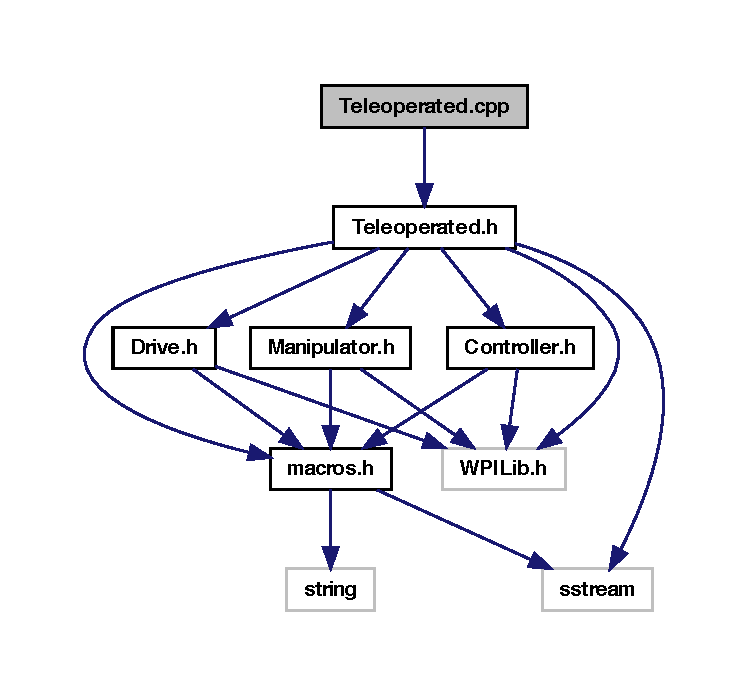
\includegraphics[width=359pt]{_teleoperated_8cpp__incl}
\end{center}
\end{figure}


\subsection{Detailed Description}
File containing definitions of functions declared in class {\itshape Teleoperated\/} (declared in \hyperlink{_teleoperated_8h}{Teleoperated.h}). \begin{DoxyAuthor}{Authors}
Matthew Haney, Drew Lazzeri 
\end{DoxyAuthor}

\hypertarget{_teleoperated_8h}{
\section{Teleoperated.h File Reference}
\label{_teleoperated_8h}\index{Teleoperated.h@{Teleoperated.h}}
}


File containing definition of {\itshape Teleoperated\/} class, which is used in the main program during Teleoperated mode to simplify things.  


{\ttfamily \#include \char`\"{}macros.h\char`\"{}}\par
{\ttfamily \#include \char`\"{}WPILib.h\char`\"{}}\par
{\ttfamily \#include \char`\"{}Drive.h\char`\"{}}\par
{\ttfamily \#include \char`\"{}Manipulator.h\char`\"{}}\par
{\ttfamily \#include \char`\"{}Controller.h\char`\"{}}\par
{\ttfamily \#include $<$sstream$>$}\par
Include dependency graph for Teleoperated.h:
\nopagebreak
\begin{figure}[H]
\begin{center}
\leavevmode
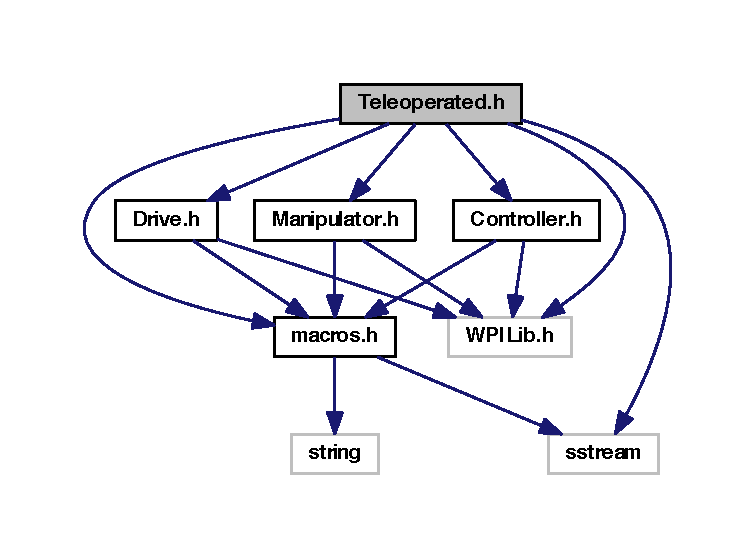
\includegraphics[width=359pt]{_teleoperated_8h__incl}
\end{center}
\end{figure}
This graph shows which files directly or indirectly include this file:
\nopagebreak
\begin{figure}[H]
\begin{center}
\leavevmode
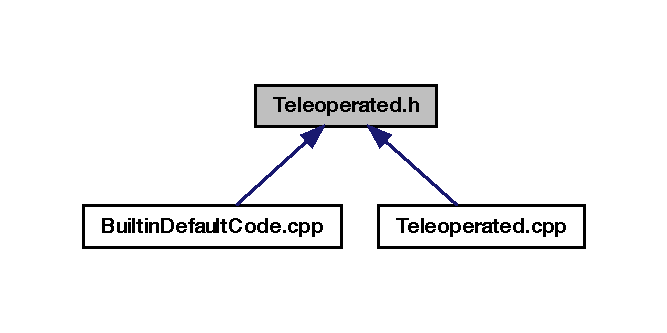
\includegraphics[width=320pt]{_teleoperated_8h__dep__incl}
\end{center}
\end{figure}
\subsection*{Classes}
\begin{DoxyCompactItemize}
\item 
class \hyperlink{class_r_j_f_r_c2011_1_1_teleoperated}{RJFRC2011::Teleoperated}
\begin{DoxyCompactList}\small\item\em Class managing robot performance in \hyperlink{class_r_j_f_r_c2011_1_1_teleoperated}{Teleoperated} mode. \item\end{DoxyCompactList}\end{DoxyCompactItemize}


\subsection{Detailed Description}
File containing definition of {\itshape Teleoperated\/} class, which is used in the main program during Teleoperated mode to simplify things. \begin{DoxyAuthor}{Authors}
Matthew Haney, Drew Lazzeri 
\end{DoxyAuthor}

\printindex
\end{document}
